%==========================================================================
%>
%>			  This is the main .tex for the 
%>				     DESIGN PHASE
%>					of PSE Group 10
%>
%=========================================================================%
\documentclass[a4paper, twoside, svgnames]{scrartcl}

% Character encoding
\usepackage[utf8]{inputenc}
\usepackage{arev}
\usepackage[T1]{fontenc}   % 8-Bit-Codierung der Fonts verwenden
  
% Page size
%\usepackage[a4paper,top=19mm,bottom=22mm,bindingoffset=10mm,left=10mm, right=15mm,heightrounded,headsep=15mm,includeheadfoot]{geometry} 
\usepackage[a4paper,top=19mm,bottom=22mm,bindingoffset=0mm,left=20mm, right=20mm,heightrounded,headsep=15mm,includeheadfoot]{geometry} 

% Color for texts and others
\usepackage{color}
\usepackage[usenames,dvipsnames, table]{xcolor}
\usepackage{etoolbox} 
%\definecolor{dark_gray}{rgb}{0.25,0.25,0.25}
  
% Customized header & footer 
\usepackage{fancyhdr}
\pagestyle{fancy}
 \fancyhf{} 	% clears all
	\fancyhead[L]{PSE Group 10 \\ Design}		% header
	\fancyhead[R]{\leftmark} 
	\fancyhead[CO]{
\includegraphics[width=0.13\linewidth]{Pictures/WHAT-Logo.png}}
	\fancyhead[CE]{
\includegraphics[width=0.1\linewidth]{Pictures/KIT-Logo.png}}
	\renewcommand{\headrulewidth}{0.5pt}
	\rhead{\nouppercase{\leftmark}}
	\patchcmd{\headrule}{\hrule}{\color{Bittersweet}\hrule}{}{}
	
	\renewcommand{\footrulewidth}{0.5pt}						% footer
	\patchcmd{\footrule}{\hrule}{\color{Bittersweet}\hrule}{}{}
	\fancyfoot[C]{\thepage}
	 
% Customized headlines
\usepackage{titlesec}
\titleformat{\subsubsection}[hang]{\bfseries\titlerule}{\thesubsubsection\enspace}{0em}{}[\titlerule]
 
\usepackage[shortlabels]{enumitem}
% \setlist{leftmargin=*}
% \renewcommand{\labelitemii}{$\circ$}
% \makeatletter
% \def\itemnumber#1{\expandafter\@itemnumber\csname c@#1\endcsname}
% \def\@itemnumber#1{\ifnum#1<10\relax0\fi\@arabic{#1}0}
% \makeatother
% \AddEnumerateCounter{\itemnumber}{\@itemnumber}{000}

%\setlist[1]{labelindent=\parindent}

% Including pictures
\usepackage{graphicx}

% Referring to tables
\usepackage{array}

% Return after CR set 0
\setlength{\parindent}{0pt} 
\setlength{\parskip}{6pt}	% space after passage



% For links of the chapters and out of the pdf + boxes around links deleted
\usepackage[colorlinks=true, linkcolor=black, urlcolor=blue]{hyperref} 
\hypersetup{
	pdftitle={Design - WHAT WareHouse Analyzing Tool},
	pdfauthor={Alexander Noe, Jonathan Klawitter, Anas Saber, Nikolaos Alexandros Kurt Moraitakis,Lukas Ehnle}}

% Glossary 
% \usepackage{ifthen}
% \usepackage{xkeyval}
% \usepackage{xfor}
% \usepackage{amsgen}
% \usepackage{etoolbox} 

% \usepackage[makeindex]{glossaries}
% \newglossaryentry{SkyServer}
{
  name=SkyServer,
  description={is a big database for astronomical data. It contains pictures
              and other information concerning astronomy and tries to 'form a 
              map of the universe
              }
}


\newglossaryentry{KIT}
{
  name=KIT,
  description={is a technological university in Karlsruhe, Baden-Württemberg, Germany 
              (Karlsruhe Institute of Technology)}
}

\newglossaryentry{log file}
{
  name=log file,
  description={is a file where a large amount of data is saved in one or another form.}
}

\newglossaryentry{.csv}
{
  name=.csv,
  description={is a file-ending which is used for log files, 
  which saves them in a standardized formatting schema.}
}

%Feel free to censor, or whatever
\newglossaryentry{browser}
{
  name=browser,
  description={A piece of software mostly used to navigate the enchanting world of the internet, and thus most commonly
used to watch illegal movies and creep your neighbours photos on facebook. Can be also used to view nice charts.}
}

\newglossaryentry{Firefox}
{
  name=firefox,
  description={A browser that is both modern and popular. Other browsers are popular too, but not modern. }
}

\newglossaryentry{Chrome}
{
  name=chrome,
  description={is a modern browser like firefox, with the notably difference being that google knows about your
creeping of your neighbour. See browser.}
}


   
% \makeglossaries   
 
 
% %Glossarverweise formatieren
% \DeclareRobustCommand\textsfgls[1]{\textsf{\textcolor{dark_gray}{#1}}}
% \renewcommand{\glsdisplayfirst}[4]{\textsfgls{#1}} % Farbe/Schriftart für das erste Vorkommen einer Referenz festlegen
% \renewcommand{\glsdisplay}[4]{\textsfgls{#1}} % Farbe/Schriftart für alle anderen Referenzen festlegen
% 
% %Glossareinträge formatieren
% \renewcommand{\glossaryentryfield}[5]{%
% \item % bullet point
% \textbf{\glstarget{#1}{#2}}% the entry name
% \space #3% the description
% \space [#5]% the number list in square brackets
% }%
%  
%  



%!!!!!!!!!!!!!!!!!!!!!!!!!!!!!!!!!!!!!!!!!!!!!!!!!!!!!!!!!!!!!!!!!!!!!!!!!!!%
\begin{document} % BEGIN BEGIN BEGIN BEGIN BEGIN BEGIN BEGIN BEGIN BEGIN
%!!!!!!!!!!!!!!!!!!!!!!!!!!!!!!!!!!!!!!!!!!!!!!!!!!!!!!!!!!!!!!!!!!!!!!!!!!!%

% Including the customized title page
\newgeometry{a4paper,top=19mm,bottom=7mm,left=15mm, right=15mm, heightrounded,headsep=15mm, includeheadfoot}
\begin{titlepage}

\vspace*{-3cm}
\begin{center}

\begin{tabular}{m{5.5cm} m{5cm} m{5.5cm}}
\arrayrulecolor{Bittersweet!90}

\begin{center}
\footnotesize{
\textbf{ Lehrstuhl für Systeme und Informationsverwaltung}
\newline

Prof.Dr.Ing. Klemens Böhm

Hoang Vu Nguyen

Marco Neumann
} 	
\end{center}
   & 
\begin{center}

   
\includegraphics[width=0.9\linewidth]{Pictures/KIT-Logo.png}
   
\end{center}    
   & 
\begin{center}
\footnotesize{
\textbf{Praxis der Softwareentwicklung (PSE)}\newline
WS 2012/2013\newline

Visualizing and Statistically Analyzing Access Behavior to Scientific Databases
}
\end{center}\\
\hline
 
\end{tabular}


\vspace*{4.6cm}

\Huge
QA \& Testing

\vspace*{1.5cm}

\normalsize

\begin{center}

   
\includegraphics[width=0.7\linewidth]{Pictures/WHAT-LogoText2.png}
   
\end{center} 


\vspace*{2.7cm}

{\color{Bittersweet}\hrule}
\vspace*{0.4cm}
 {\today}
 
\vspace*{0.4cm}
\normalsize

 

\begin{tabular}{r l}

\arrayrulecolor{Bittersweet!90}
\hline
& \\
 
  	Functional Specification
&
	\textbf{Alexander Noe}
\\ 
	Design
& 
	\textbf{Jonathan Klawitter}
\\ 
	Implementation 
& 
	\textbf{Anas Saber}
\\
	QA / Testing 
&
	\textbf{Nikolaos Alexandros Kurt Moraitakis}
\\
	Final 
&	\textbf{Lukas Ehnle}\\

 
\end{tabular}

E-M@il: \href{mailto:pse10-group14-ws12@ira.uni-karlsruhe.de}{pse10-group14-ws12@ira.uni-karlsruhe.de}
% Bottom of the page

\end{center}
\end{titlepage} 
\restoregeometry
\newpage 

%\vspace*{0.1cm}
\tableofcontents
  
\newpage 
\section{Architecture}

WHAT is based upon a intransparent multitier architecture. 
The GUI, presentation logic, application processing, data accessing and storing data
are logically and also partly locally separated. Intransparent means that communication
between tiers just happens between adjacent ones. The different tiers are described below.


\begin{center}
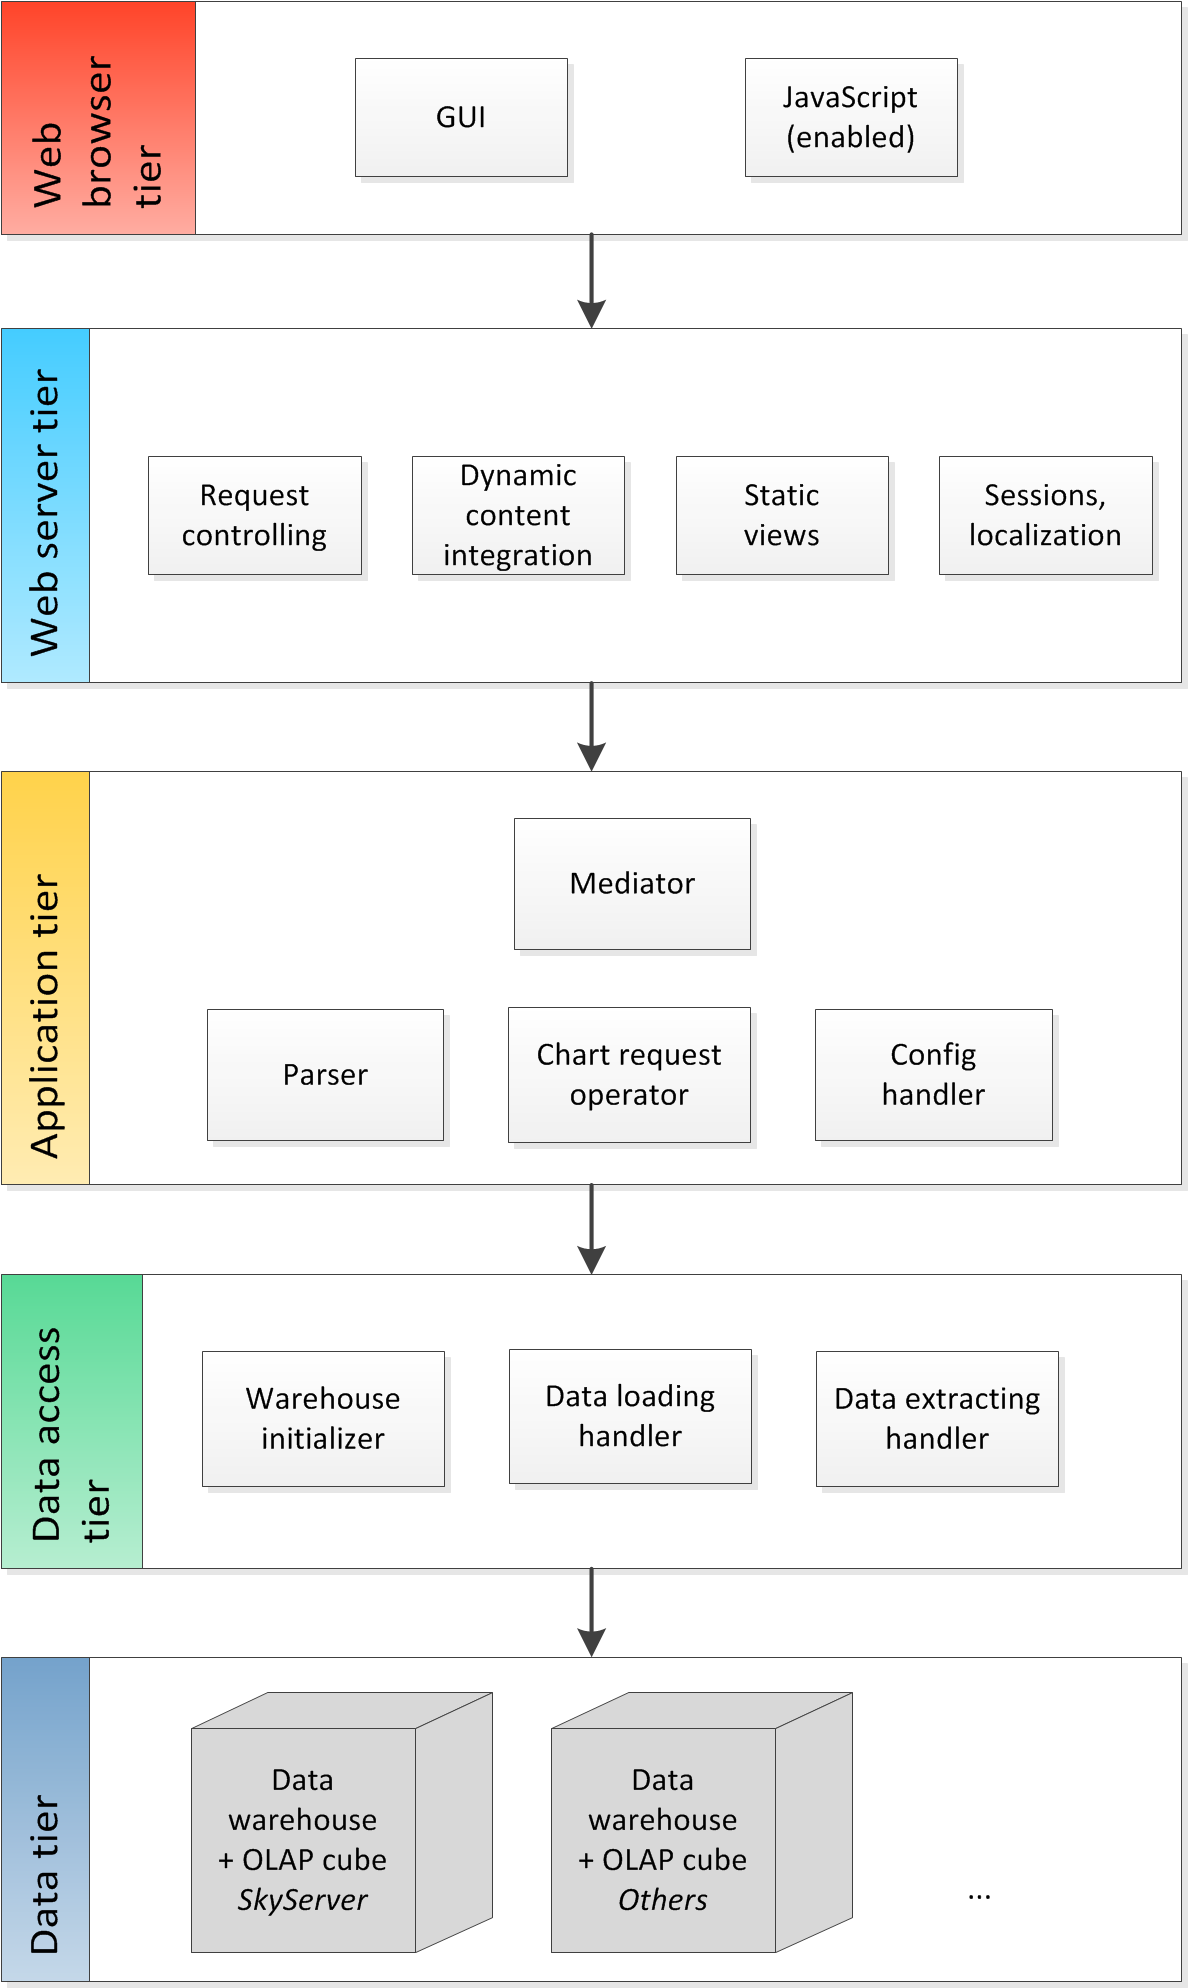
\includegraphics[width=0.6\linewidth]{Pictures/TierArchi.png} 
\end{center}   


\subsection{Web browser tier}
The web browser tier represents the web browser of the client on which the GUI, a web page, will be displayed.
As the web page uses JavaScript, it has to be enabled in the browser. 
Besides this, Google Chrome and Firefox have to be supported. 


\subsection{Web server tier}
The web server provides the presentation logic. This includes static html-pages and integration of dynamic
content. Other tasks are sessioning, localization (languages) and most important request controlling. 
Which means it handles the actions triggered on the web page and decides whether it can handle them itself 
or pass them to application tier. Last one happens for example when a chart is requested. 
The Java Play framework is used in this tier.


\subsection{Application tier}
In the application tier the parsing process, managing the configuration files and above all 
chart request managing are taking place. 

\subsection{Data access tier}
This tier manages all requests of loading and extracting data from the data tier. So its main task is
to build a bridge from the application in Java to the SQL language of the Oracle warehouses and OLAP-Cubes.
If there is enough time to implement this optional function, it will also handle 
the automatic initialization of new data warehouses.  

\subsection{Data tier}
In the data tier the data warehouses and their OLAP-Cubes are stored. 
This will be done with the Oracle software.  


\section{Web page design}


\begin{center}
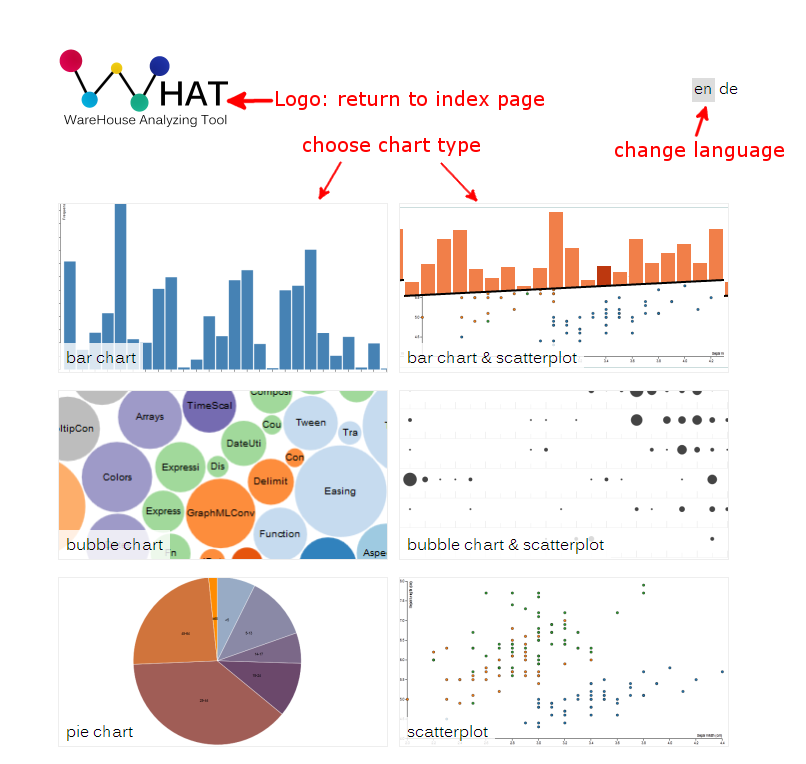
\includegraphics[width=0.9\linewidth]{Pictures/WHATHome.png}
\end{center}   

This is a prototype webpage, to show how the GUI could look like. It is not yet complete.
There will be an admin login to access a password protected page where you can alter
some settings of the GUI, but its main purpose is to allow the admin to initialize the data warehouse
with skyserver logfiles %or just plain logfiles? not skyserver specific?

\section{Classes}



\subsection{Server tier class diagram}
This diagram shows the webserver tier of wHAT. It controls the webserver and it can only access the facade of the tier below.
\begin{center}
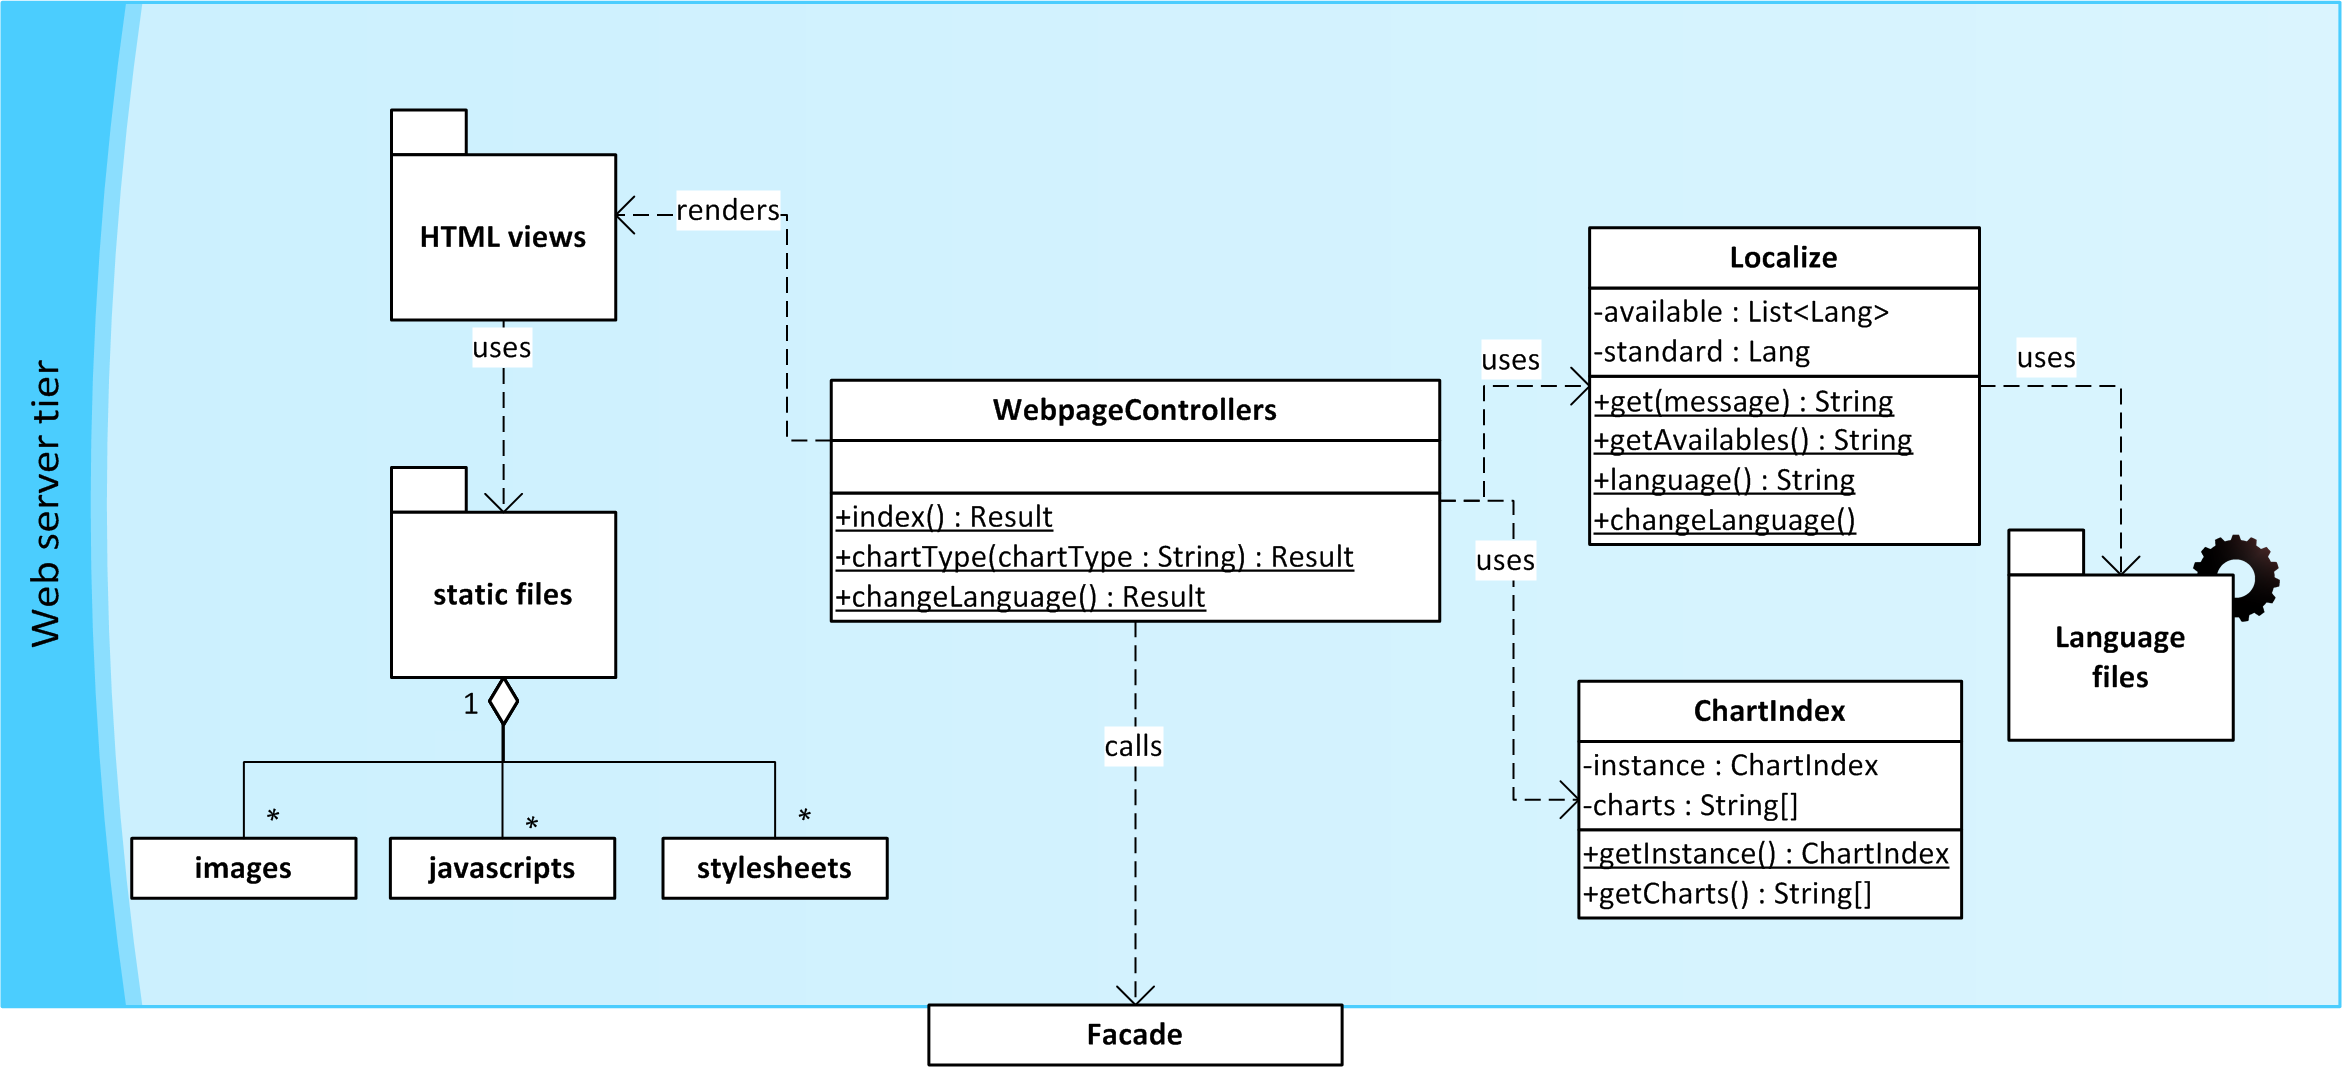
\includegraphics[width=1\linewidth]{Pictures/ServerTierDia.png}
%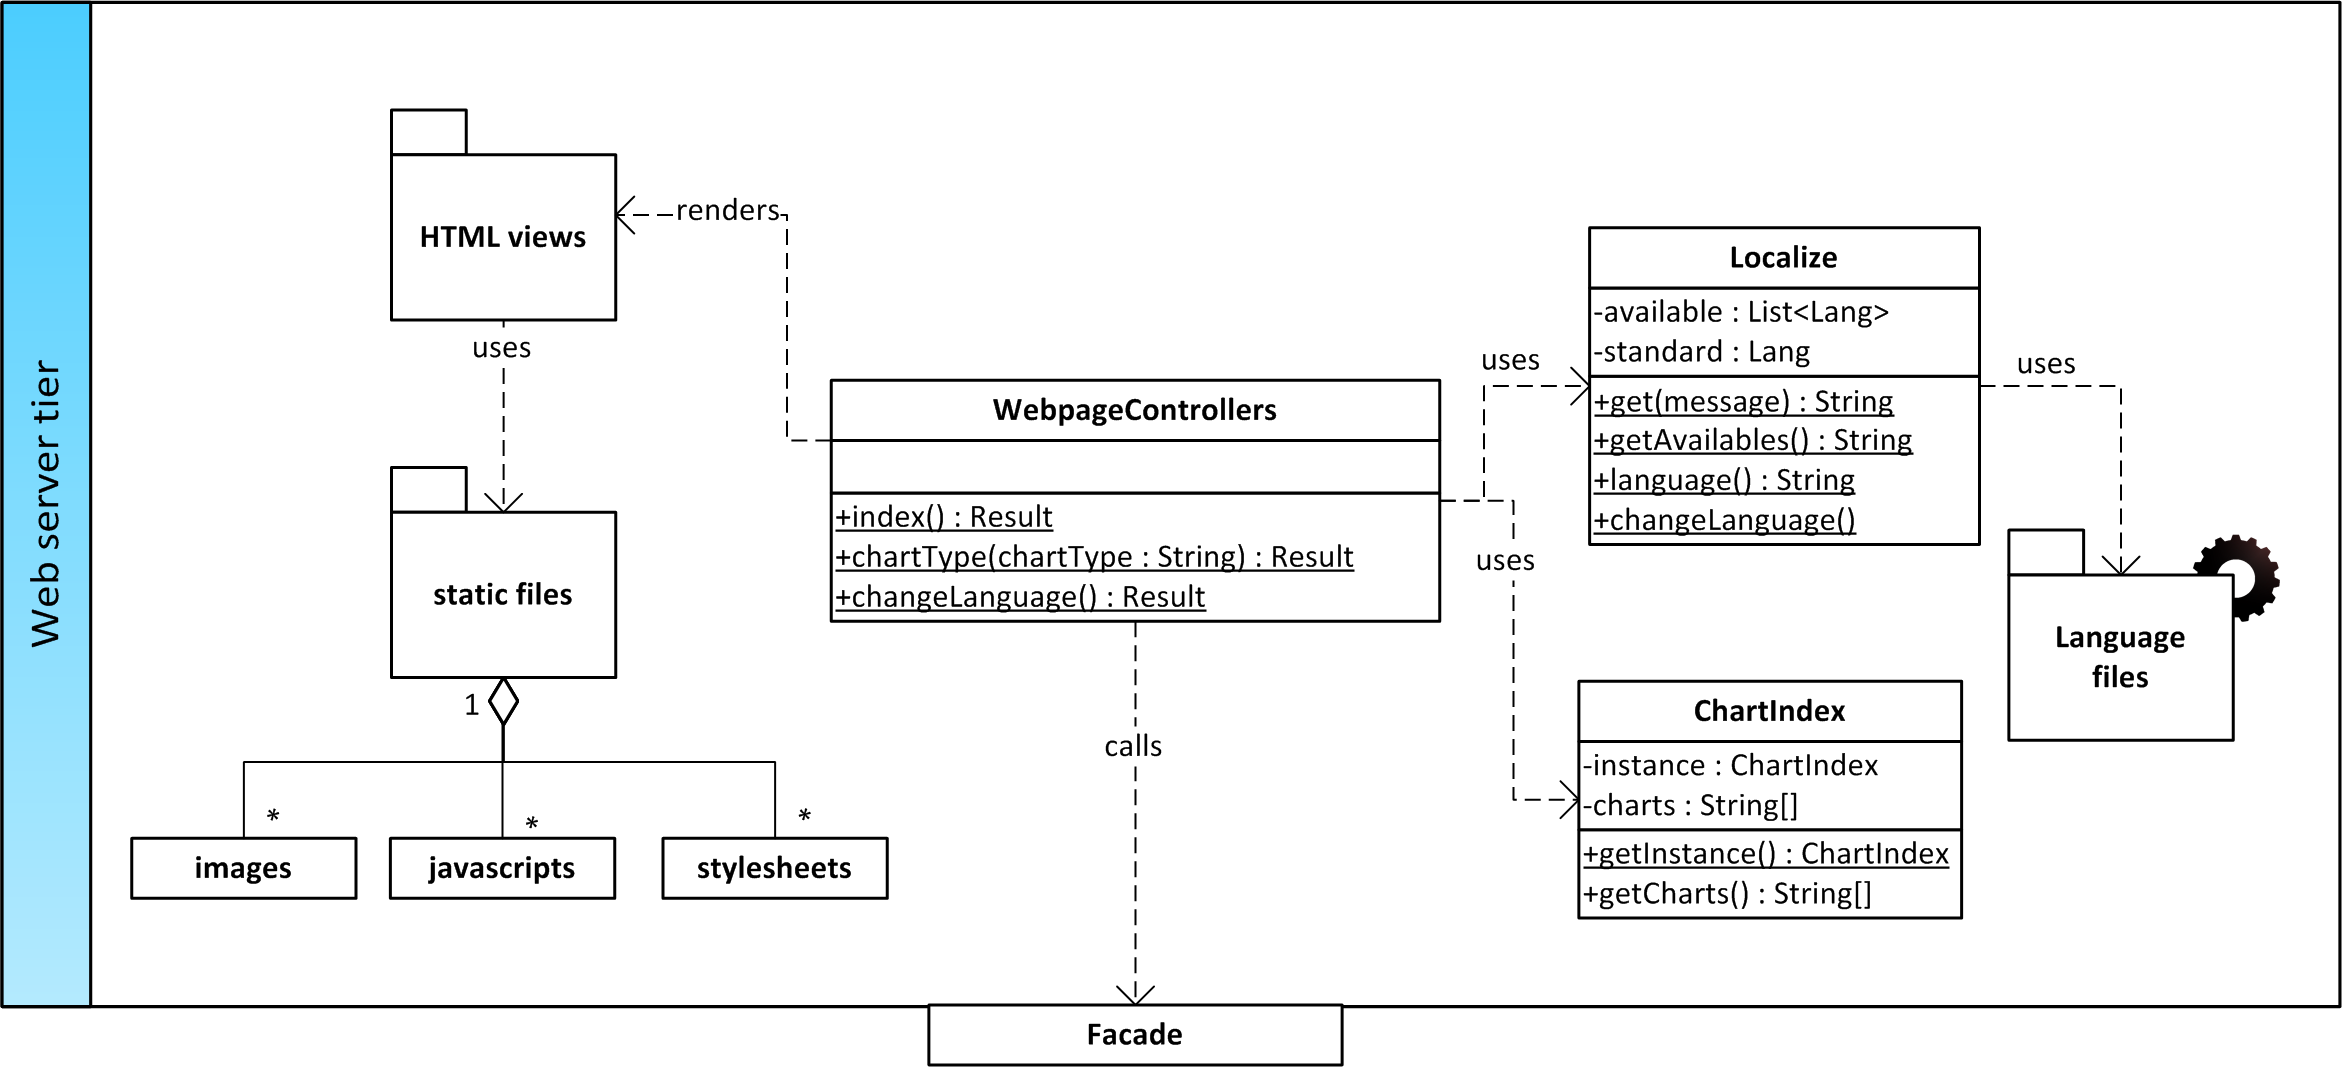
\includegraphics[width=1\linewidth]{Pictures/ServerTierDiaNormal.png} 
\end{center}   


\subsubsection*{WebpageControllers}
All valid HTTP requests are mapped to a method from WebpageControllers.
WebpageControllers either uses other helper classes to handle requests itself  
or makes calls to the facade of the application tier. 
The last step done by WebpageControllers is to create a valid HTTP response.
                                                                            

\subsubsection*{HTML views}
The HTML views contain the main template for, and all other HTML content of the webpage. %unklar
They do not have to be static, but can also dynamically integrate some content, e.g. localized strings.

\subsubsection*{Static files}
Static files contains all files of the webpage, which are not changed during runtime. 
This includes, but is not limited, to images of the webpage, javascript files and stylesheets.

\subsubsection*{Localize}
Localize is a static helper class handling all the language related things. 
It has a method to get localized Strings using the language files, 
to change the language of the webpage und methods determining all available languages, 
%dieser Satz, passt der syntaktisch? Sollte es methods sein?
so they can be integrated in the webpage once they are present.

\subsubsection*{ChartIndex}
ChartIndex implements the singleton pattern. On instantiation it scans which chart types are available 
and saves them internally. This is used by the index page to dynamically display all available chart types,
even if one is deleted or added.
%Do we have to specify how one might add them? I mean, not here, but somewhere.


\subsection{Application \& Data access tier class diagram}
This is the application tier for the analyzer-part of WHAT. 
\newpage
\begin{center}
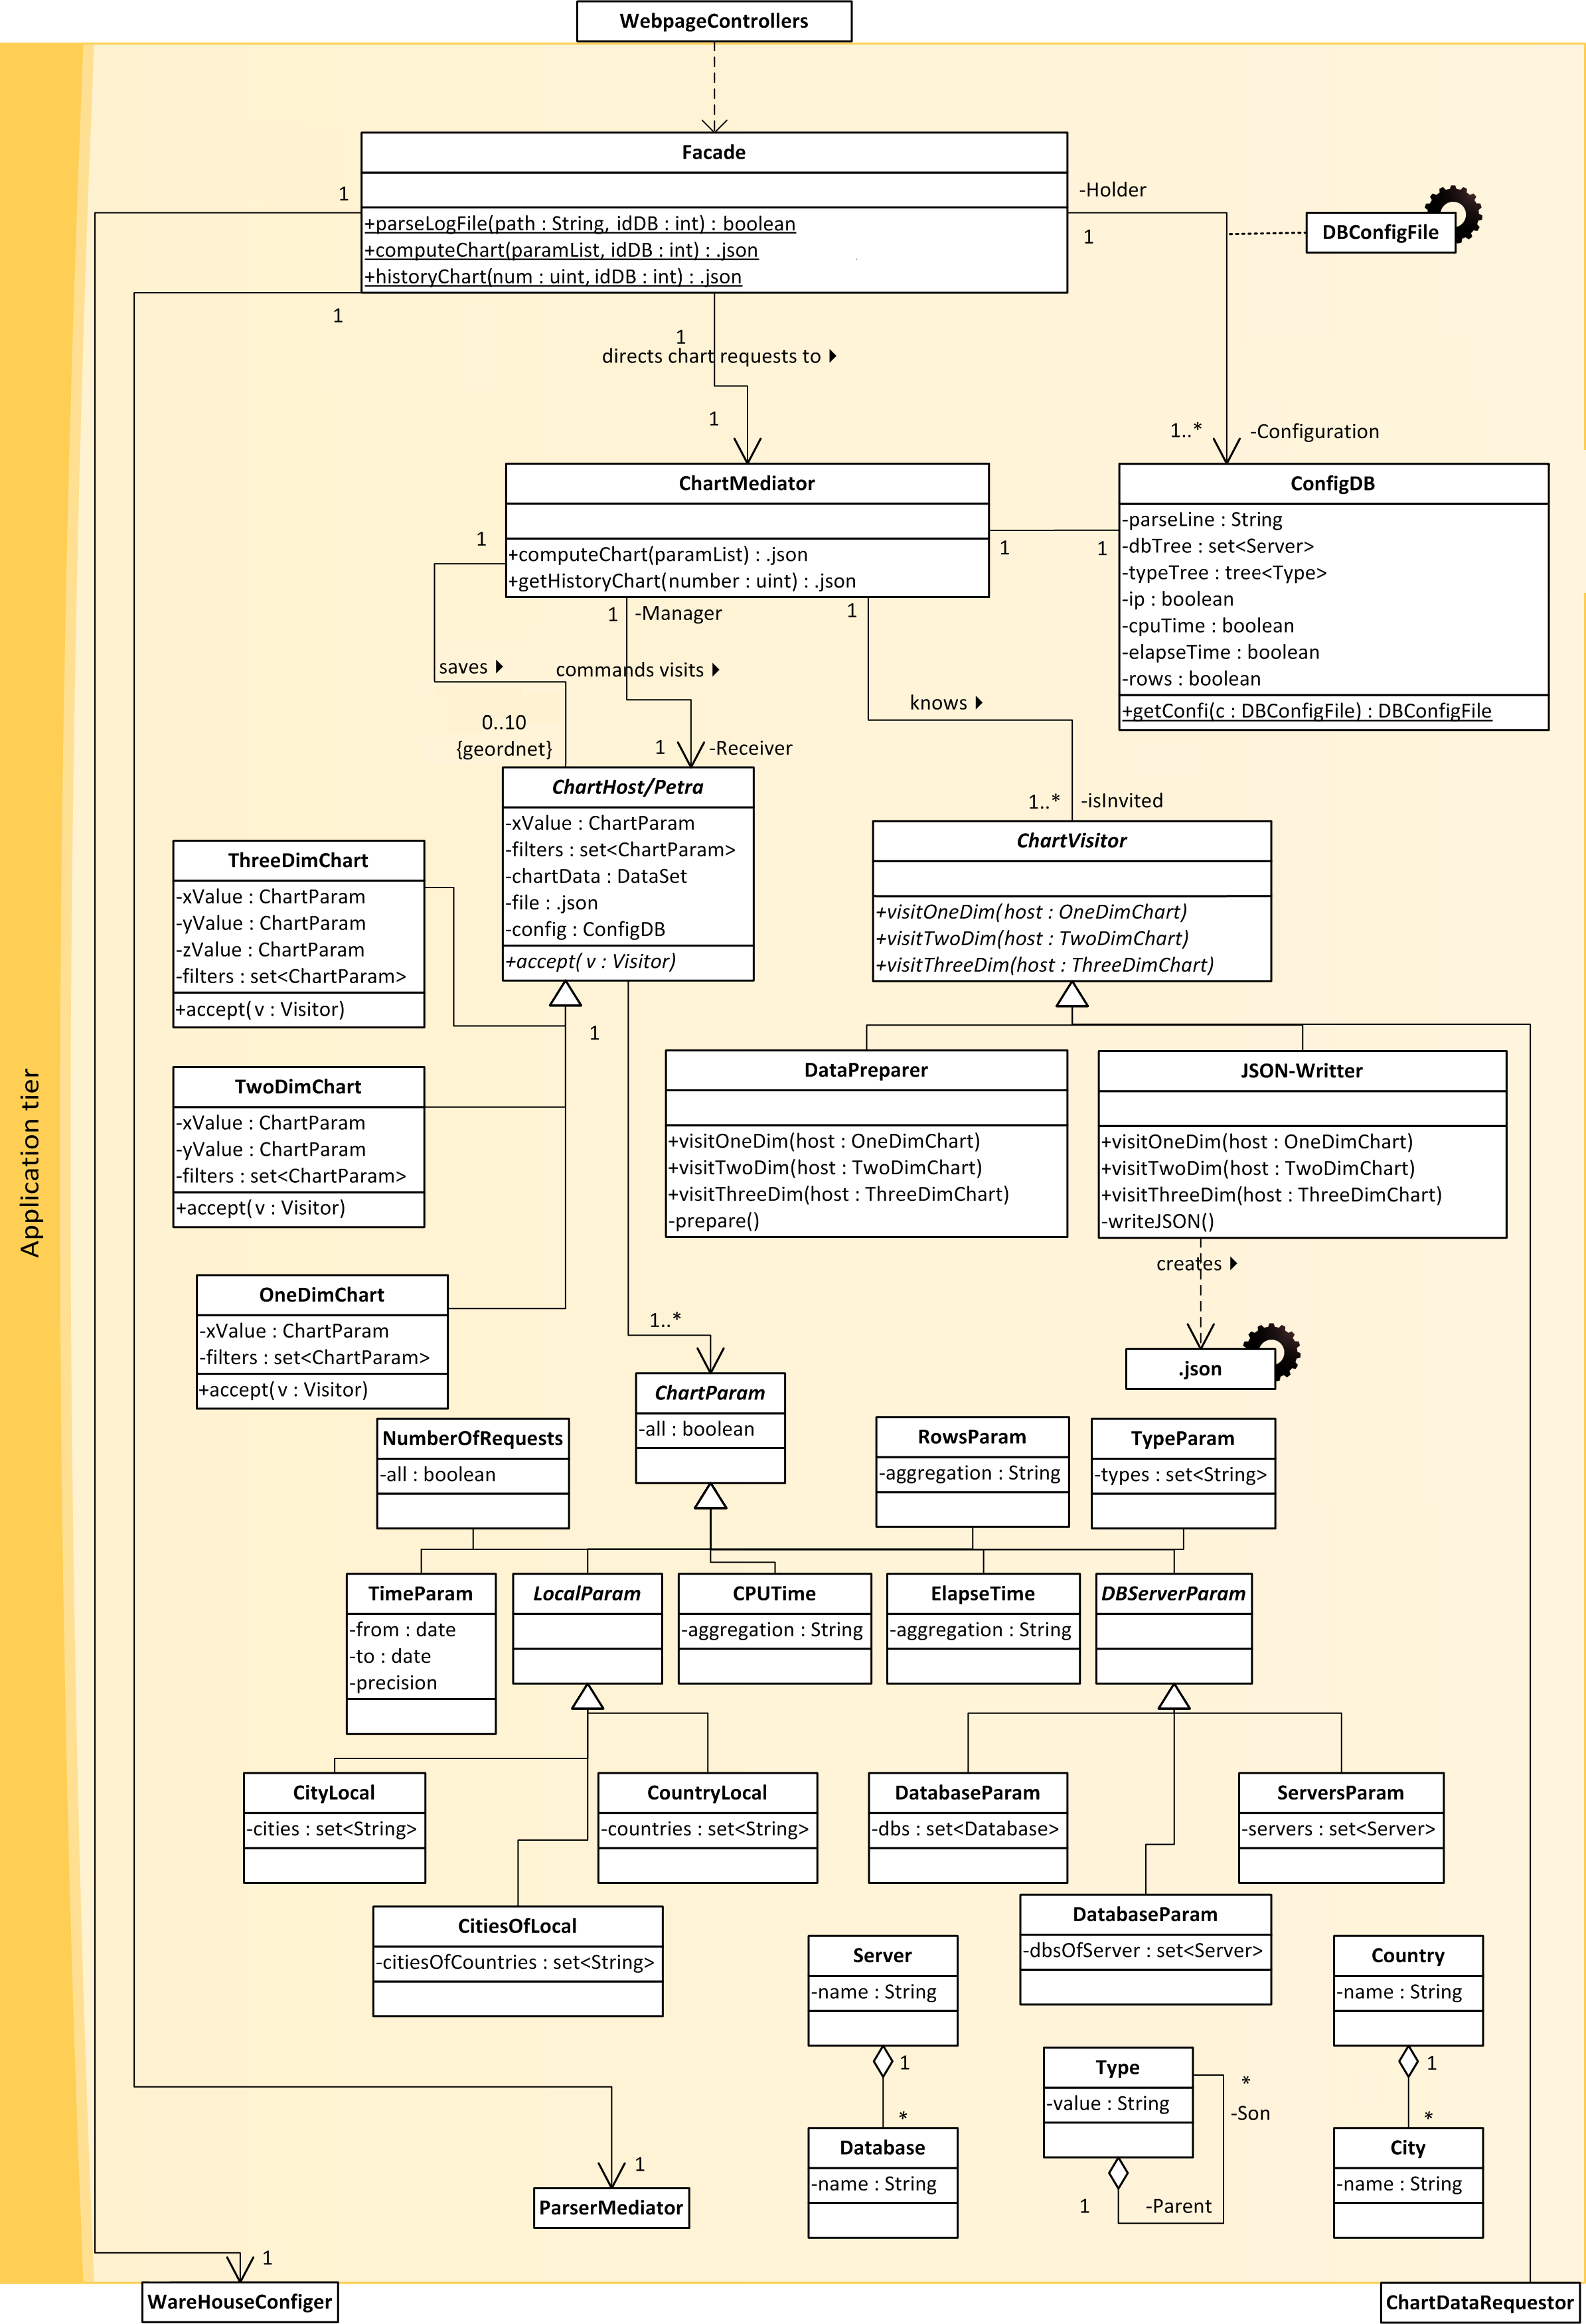
\includegraphics[width=0.9\linewidth]{Pictures/AppTierDia1.png}
%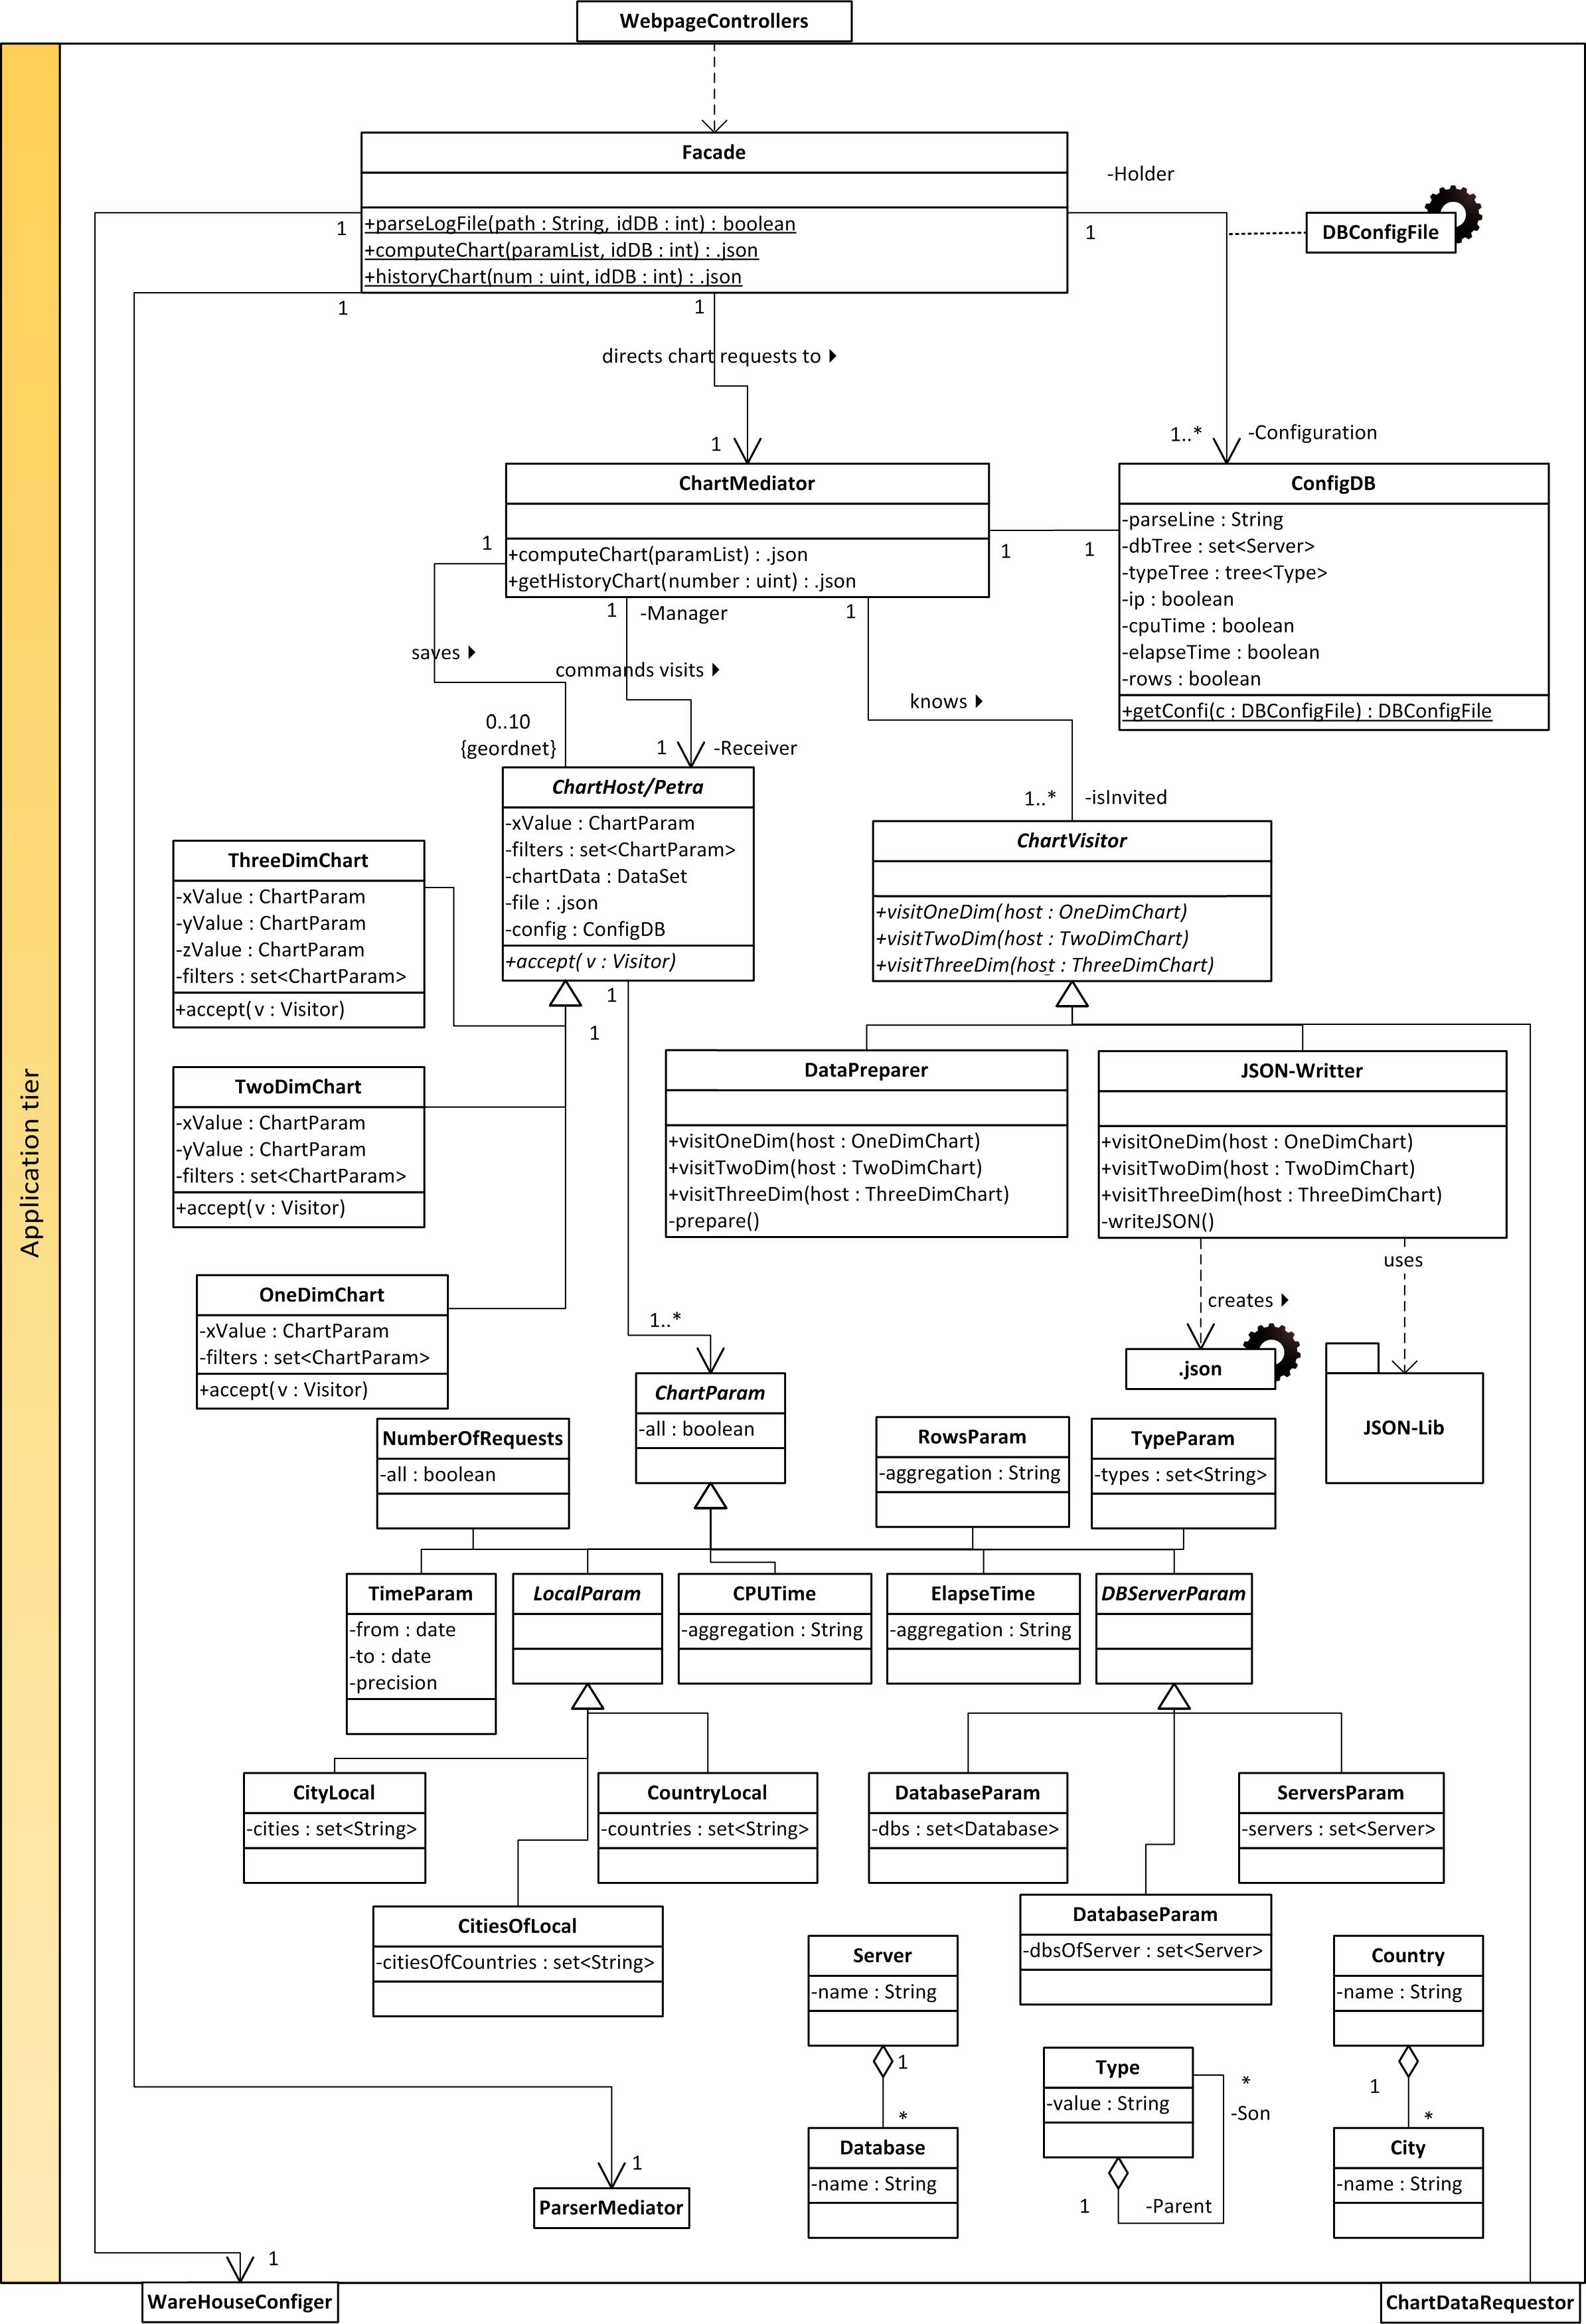
\includegraphics[width=0.9\linewidth]{Pictures/AppTierDia1Normal.png} 
\end{center}  

This is the design for the parser. 

\begin{center}
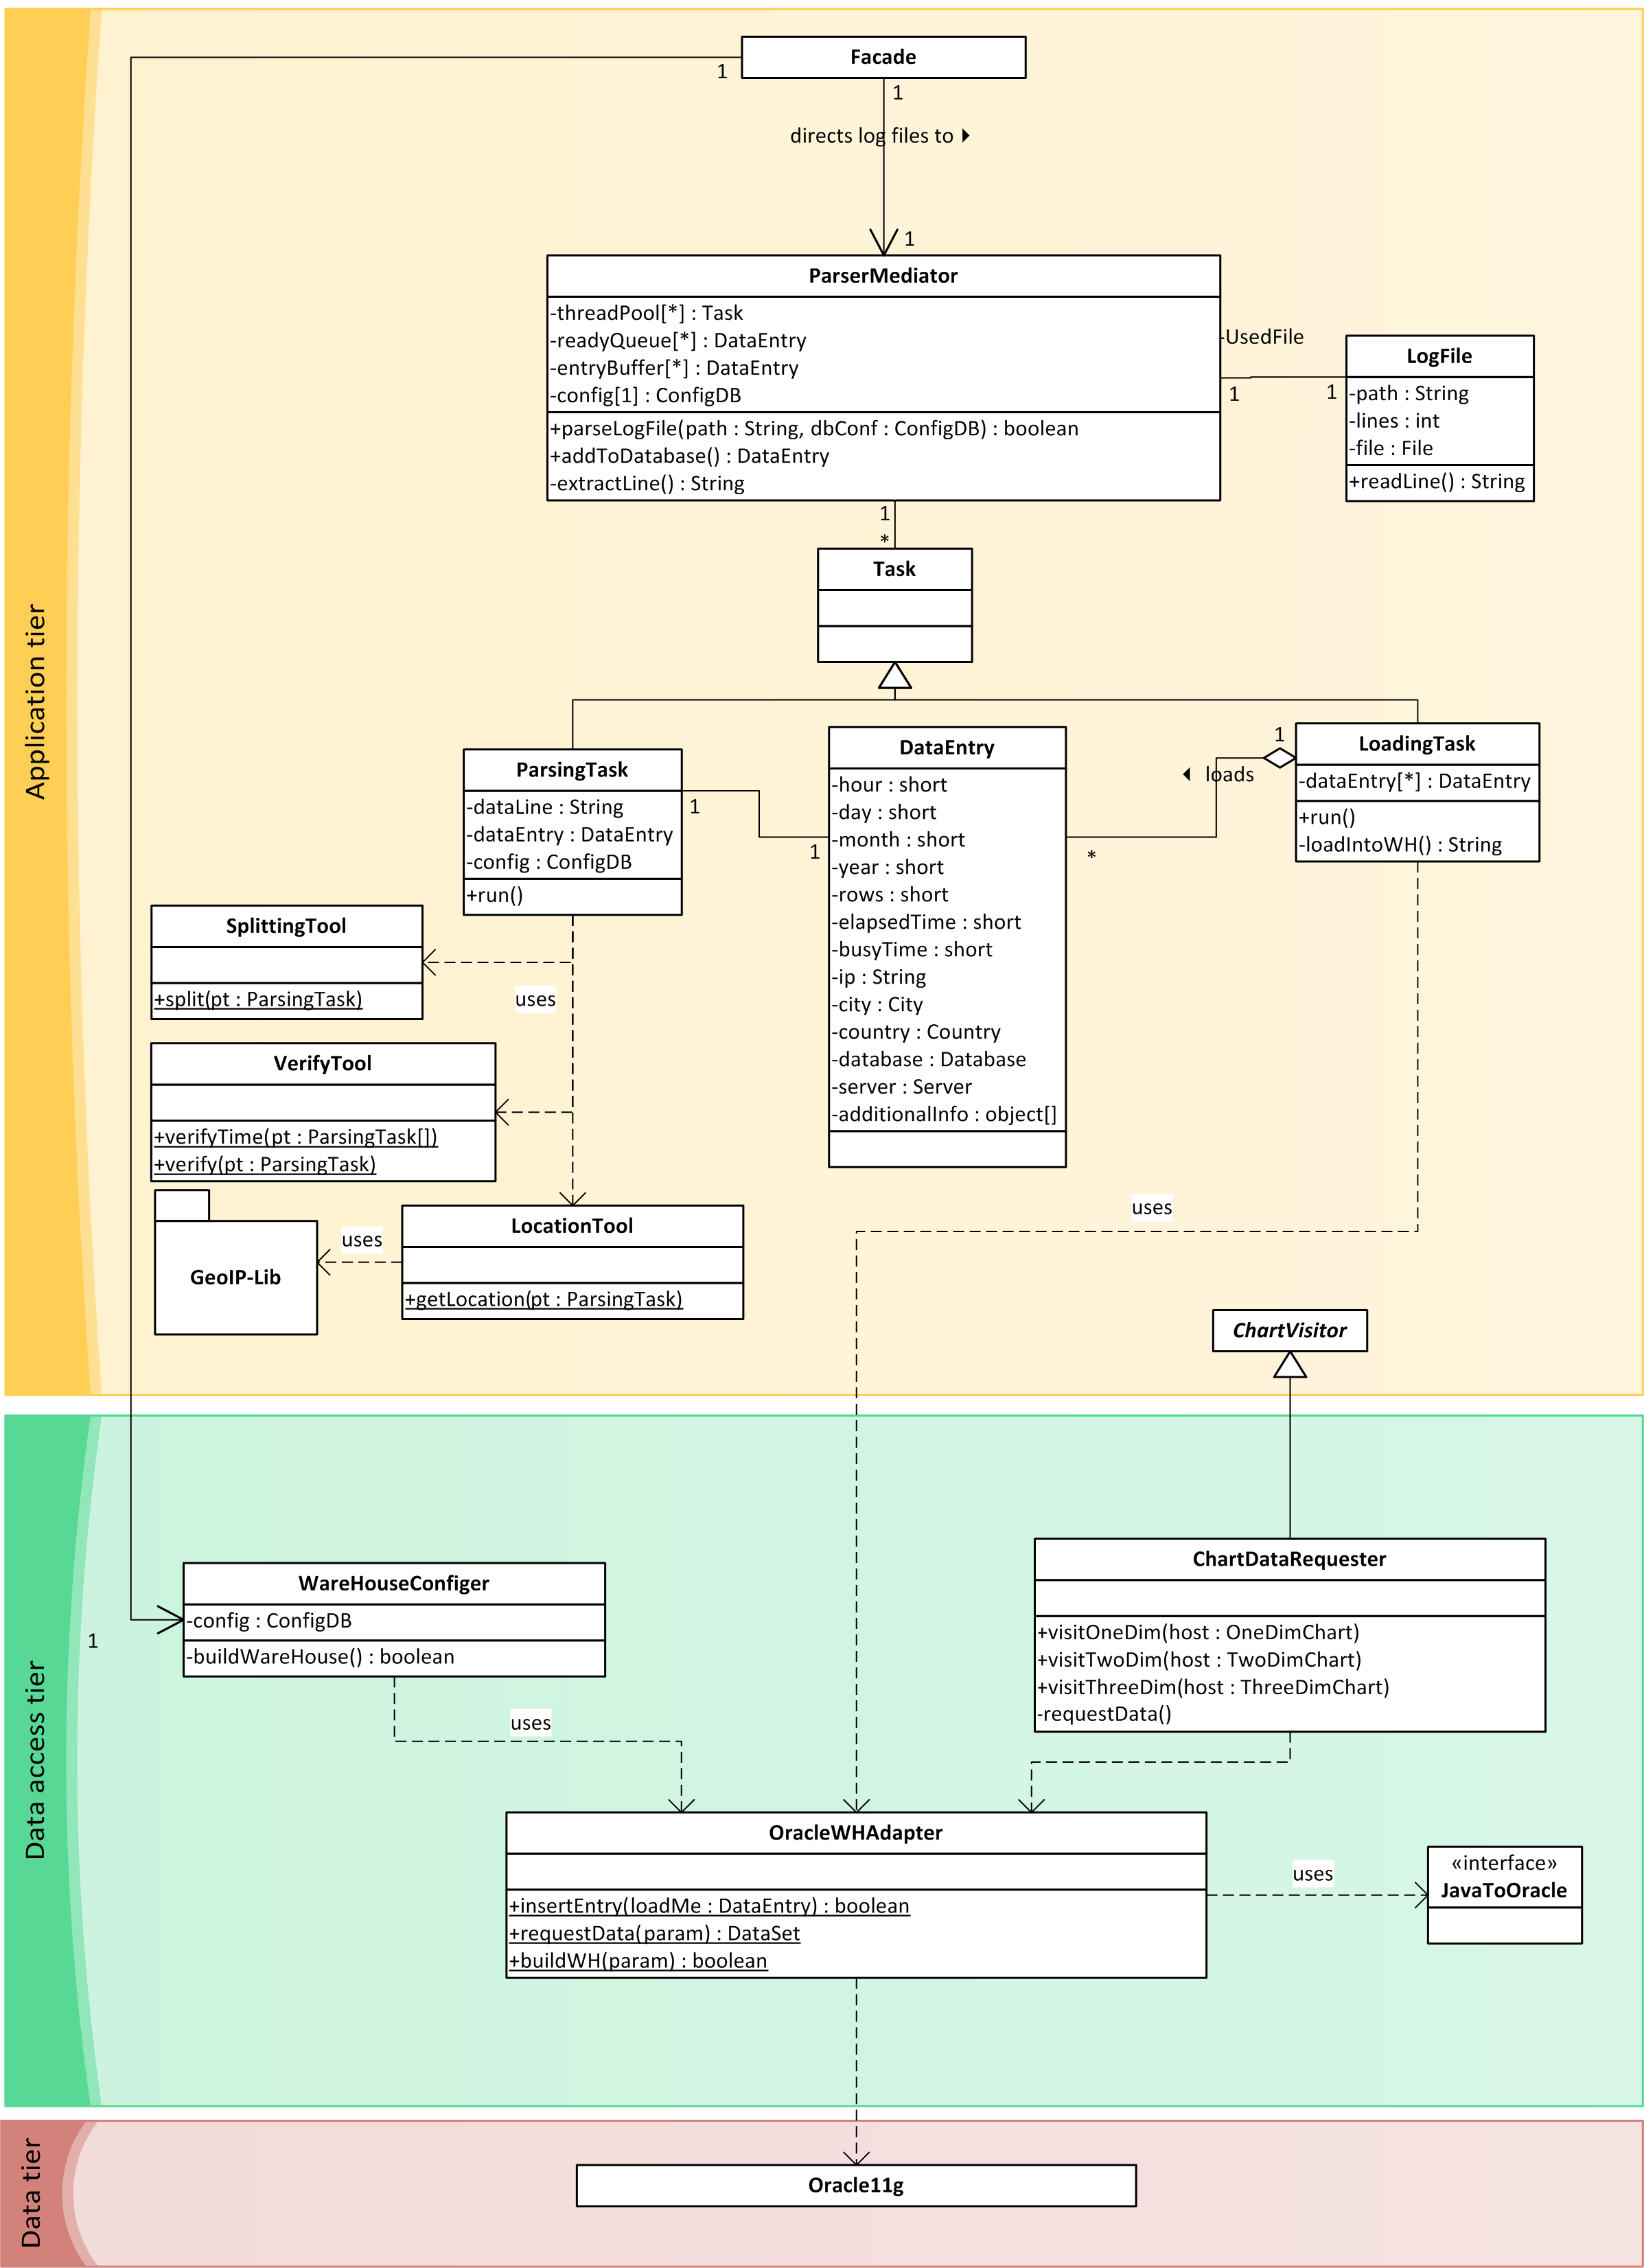
\includegraphics[width=0.9\linewidth]{Pictures/AppTierDia2.png}
%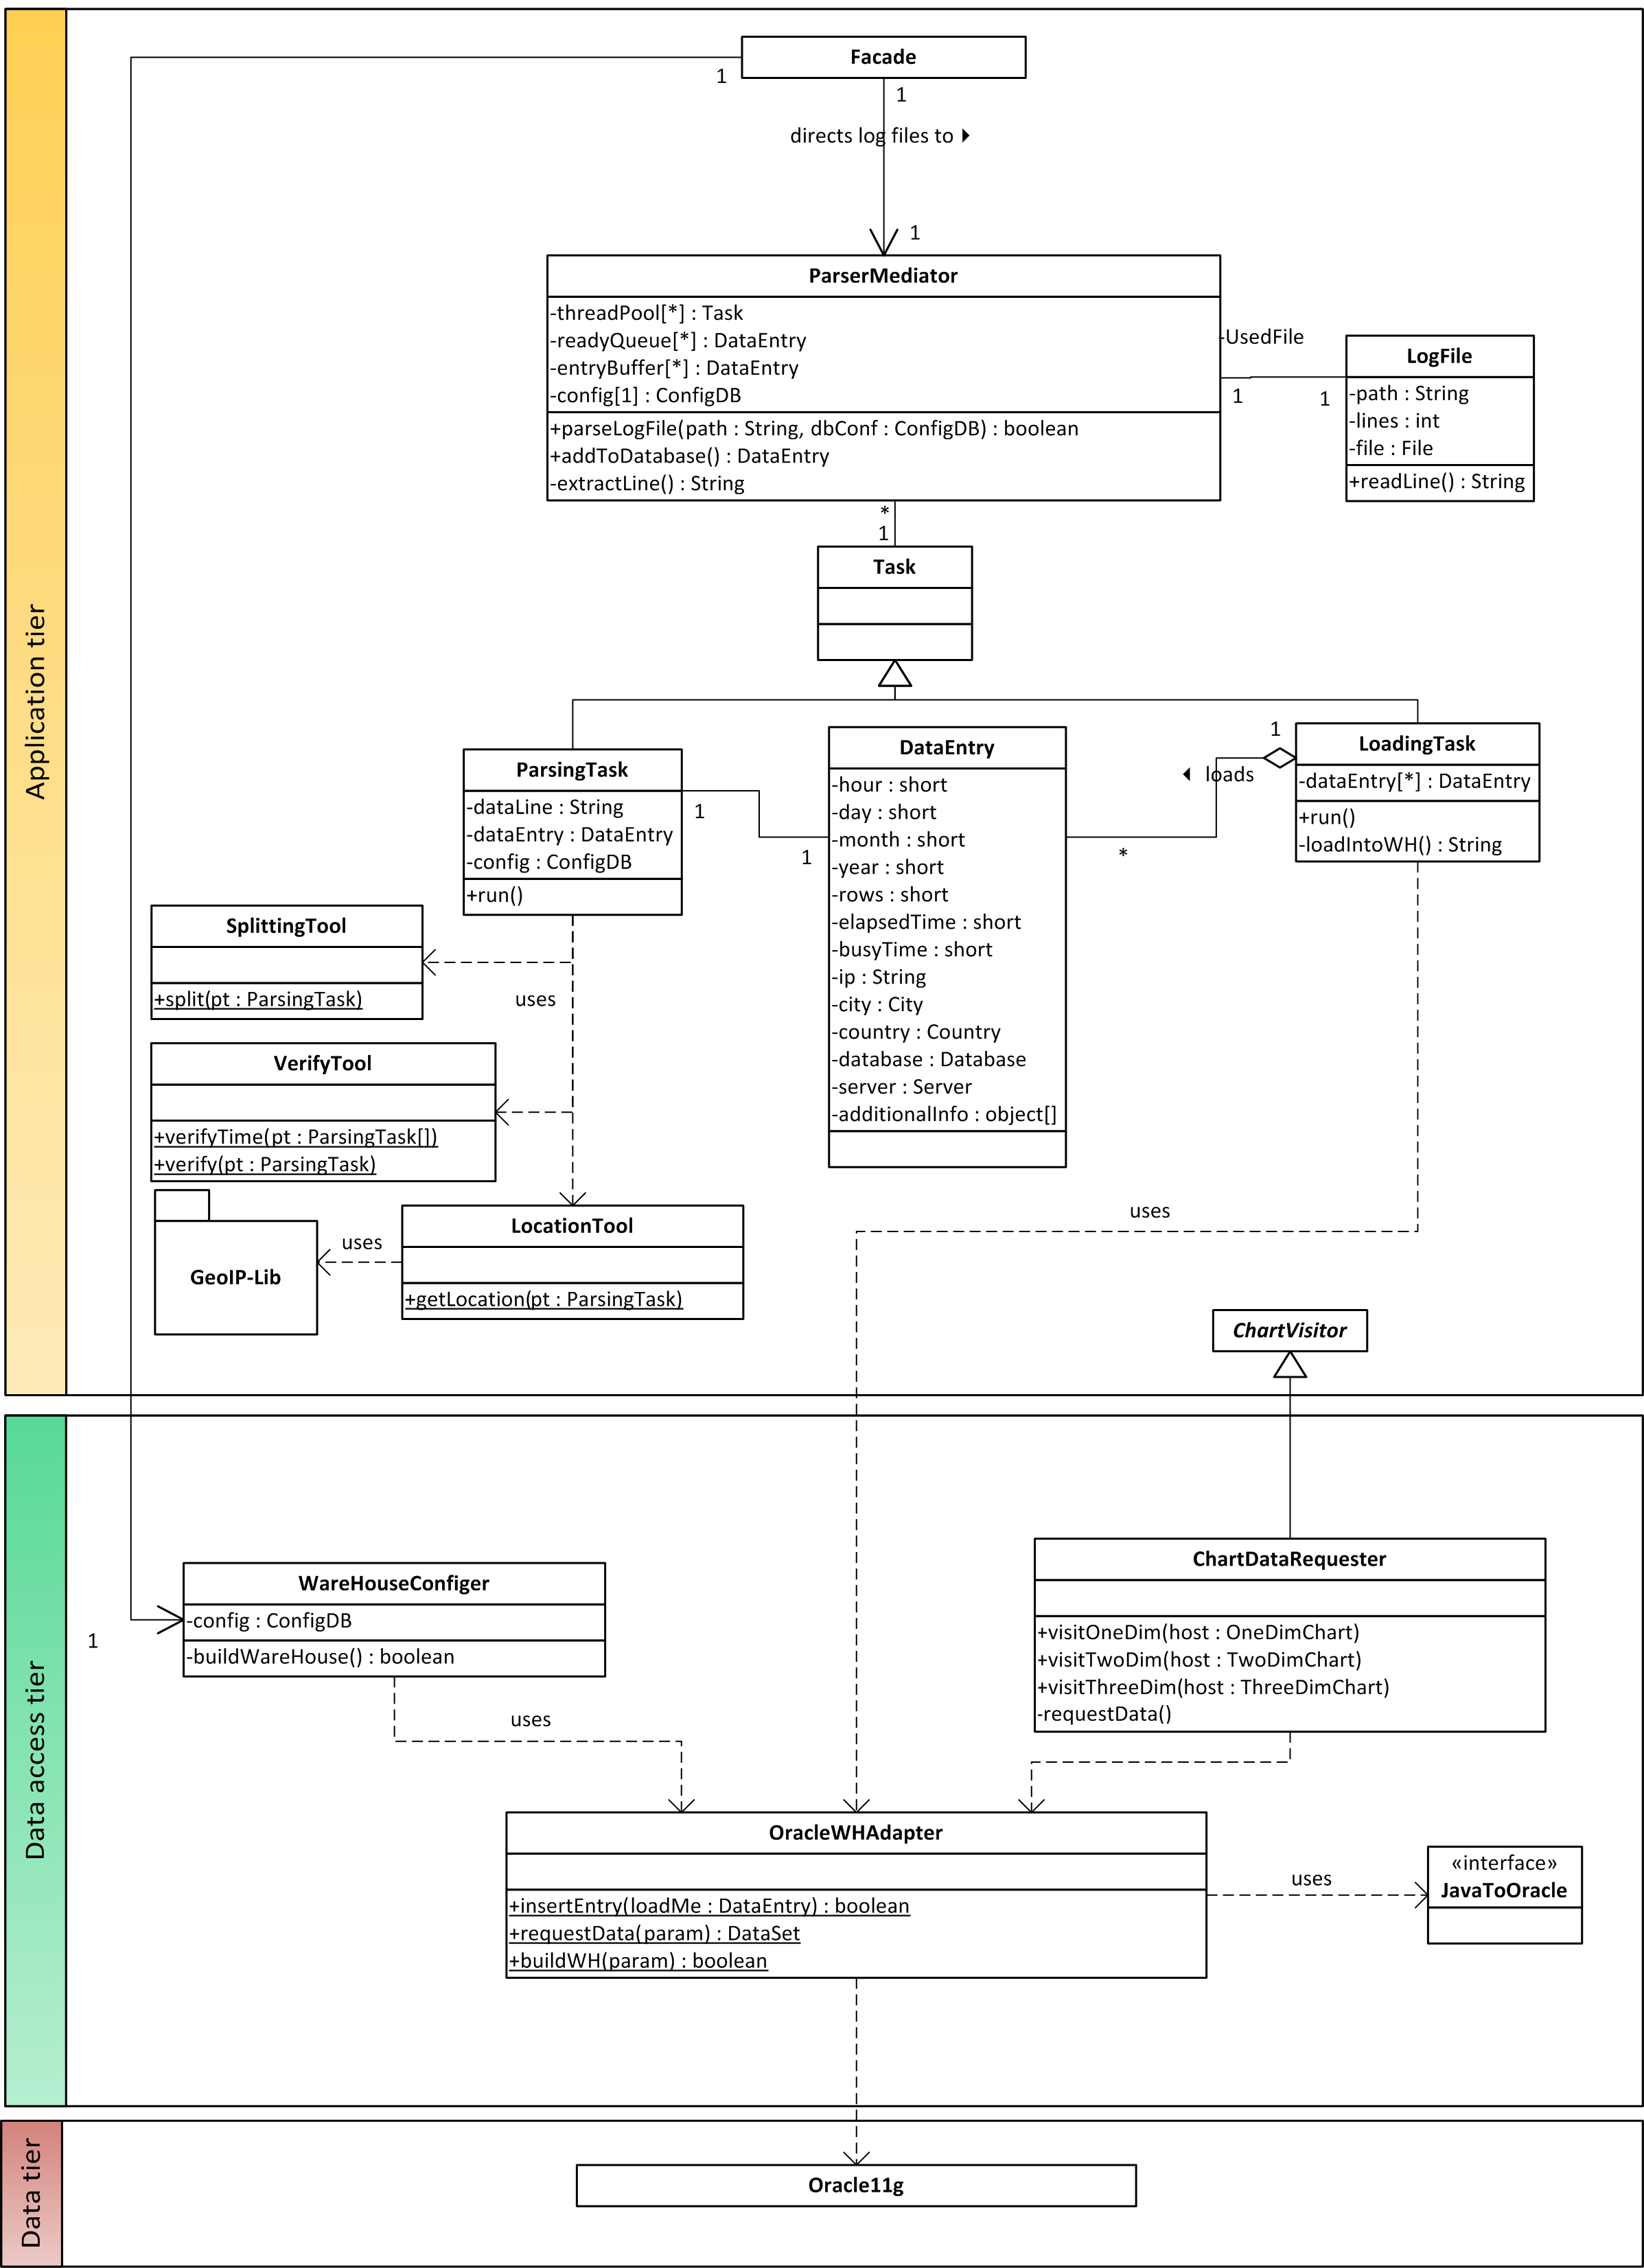
\includegraphics[width=0.9\linewidth]{Pictures/AppTierDia2Normal.png} 
\end{center}  

\subsection{Facade + Configurations}

\begin{center}
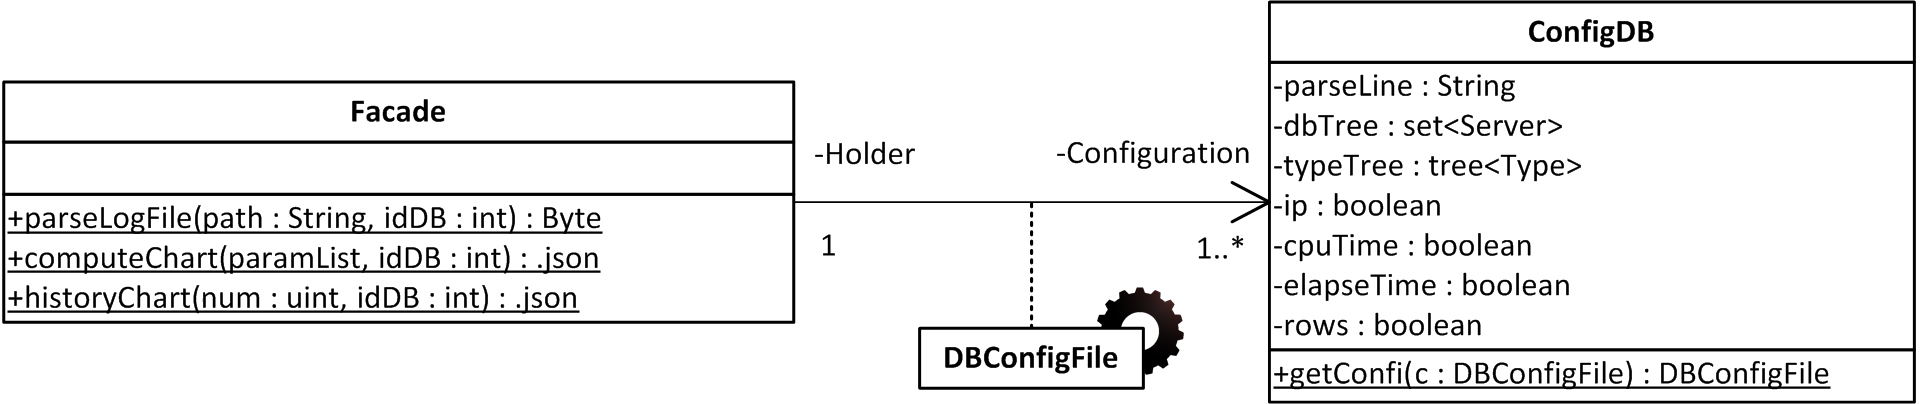
\includegraphics{Pictures/Parts/FacadeConfi.png}
\end{center}   

\subsubsection*{Facade}
\subsubsection*{ConfigDB}

\begin{center}
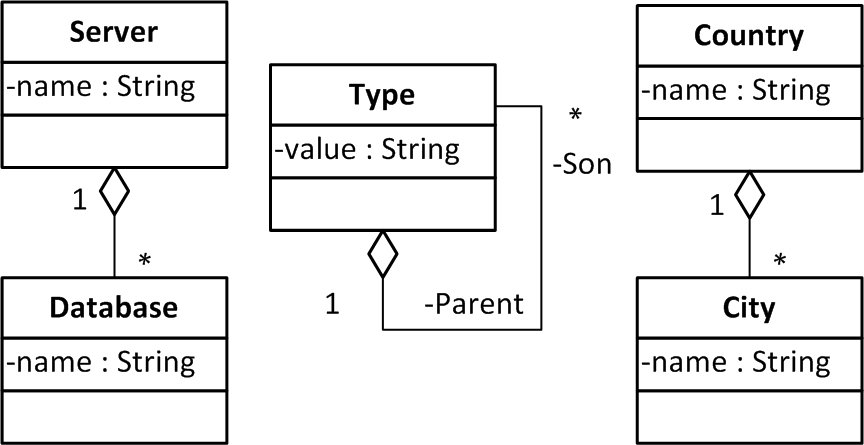
\includegraphics{Pictures/Parts/Strings.png}
\end{center}  
\subsubsection*{Server, Database}
\subsubsection*{Type}
\subsubsection*{Country, City}


\subsection{Chart request operator}
Visitor pattern blabla   
classes
\begin{center}
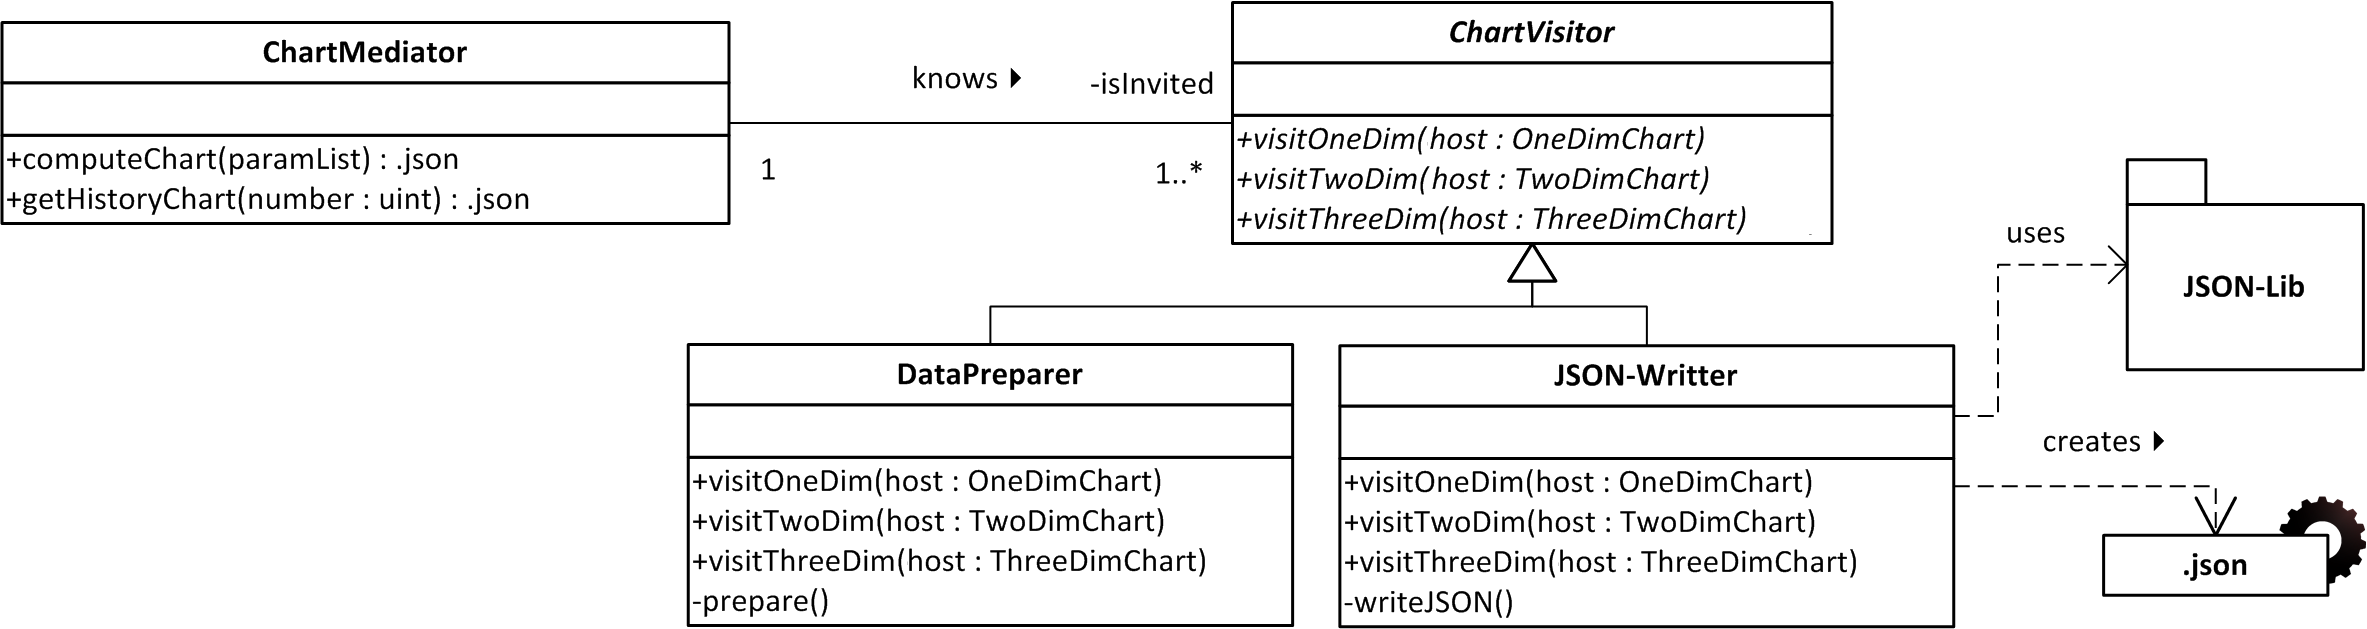
\includegraphics[width=1\linewidth]{Pictures/Parts/MediVisi.png}
\end{center}  
\subsubsection*{ChartMediator}
\subsubsection*{ChartVisitor}
\subsubsection*{DataPreparer}
\subsubsection*{JSON-Writter}
\subsubsection*{.json}
\subsubsection*{JSON-Lib}


\begin{center}
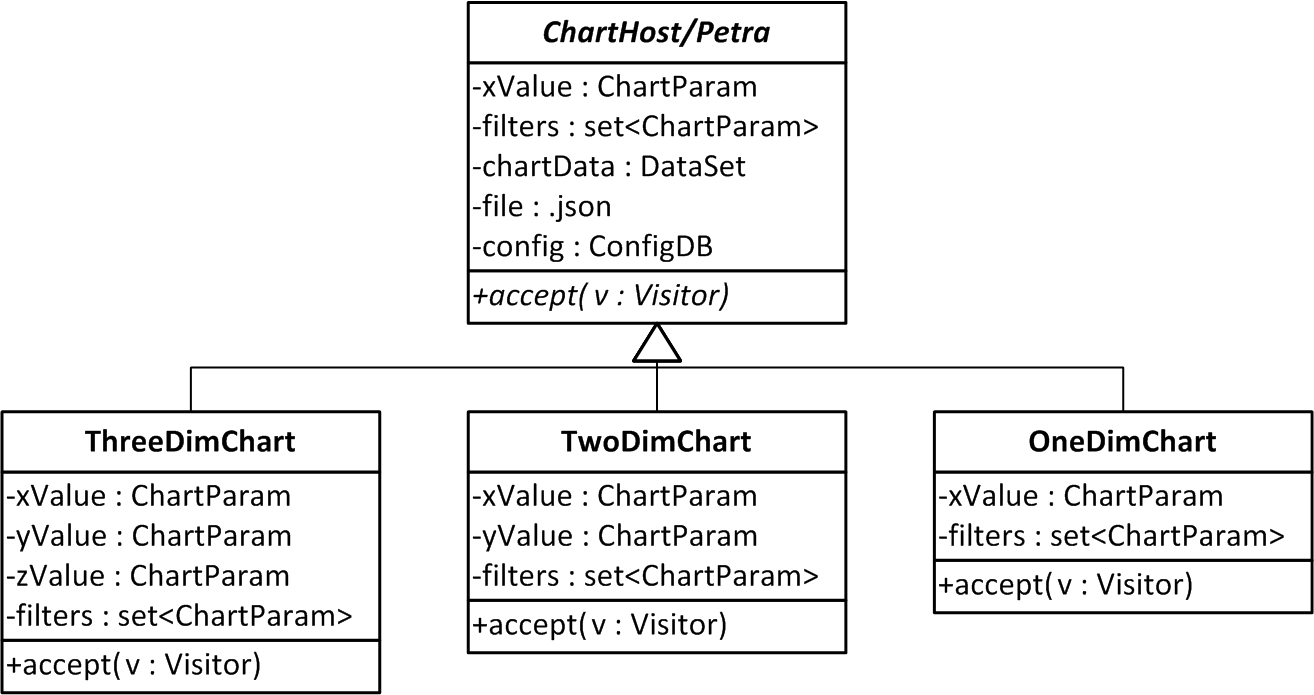
\includegraphics{Pictures/Parts/Petra.png}
\end{center}  
\subsubsection*{ChartVisitor}
\subsubsection*{OneDimeChart}
\subsubsection*{TwoeDimeChart}
\subsubsection*{ThreeDimeChart} 


\subsection{Chart parameters}
\begin{center}
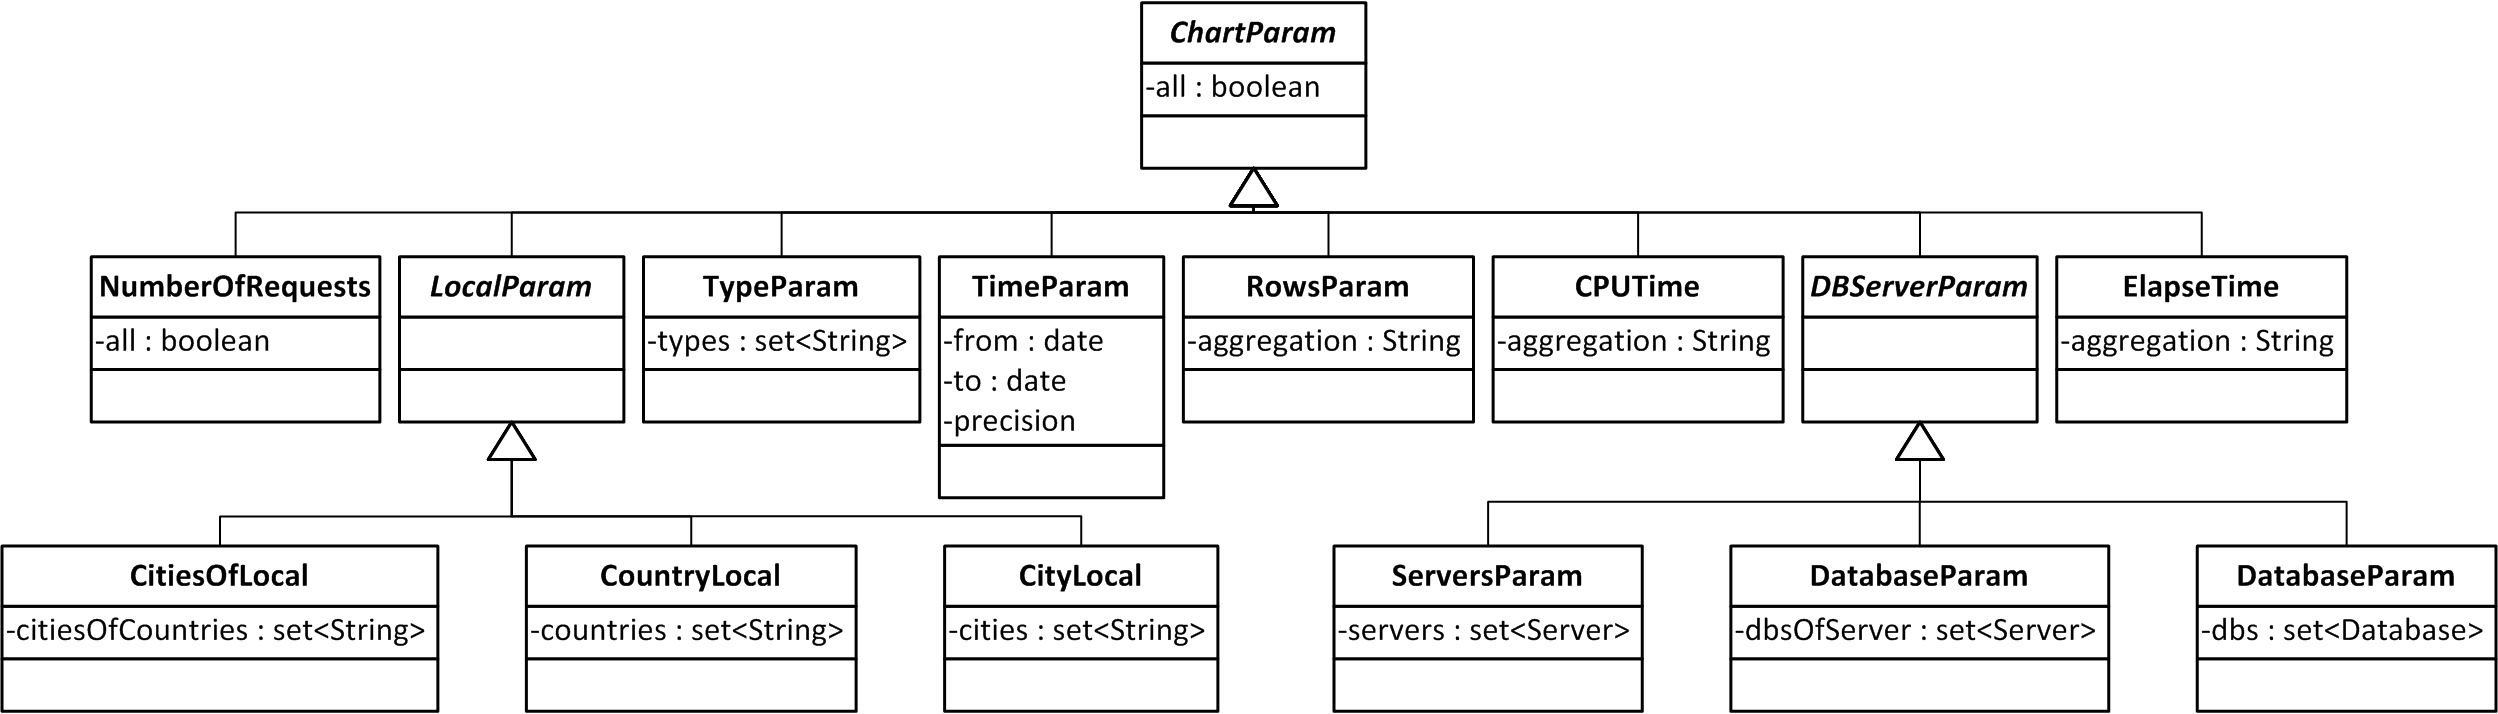
\includegraphics[width=1\linewidth]{Pictures/Parts/ChartPara.png}
\end{center}  
\subsubsection*{ChartParam} 



\subsection{Parser}

\begin{center}
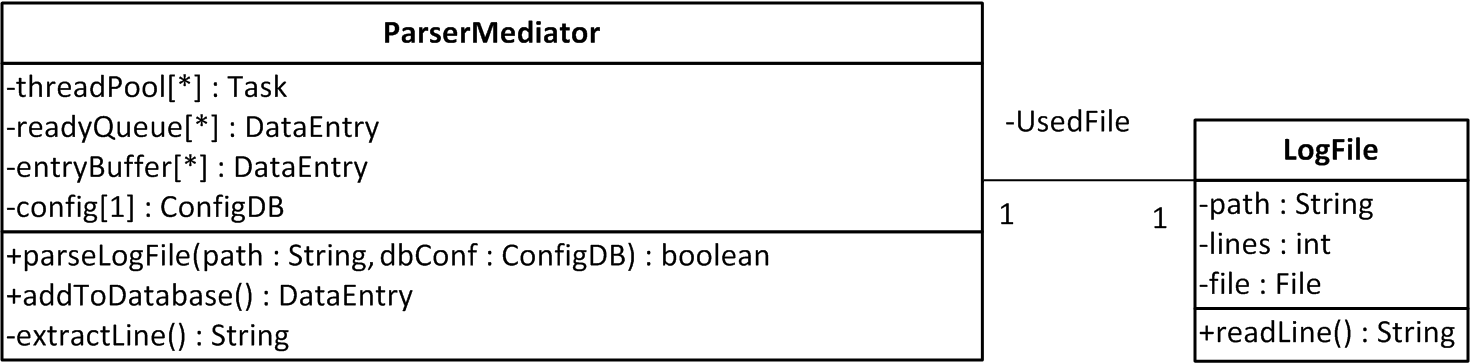
\includegraphics{Pictures/Parts/ParsMedi.png}
\end{center}  

\subsubsection*{ParserMediator}
ParserMediator is the 'main'-Class of the Parser. It creates and administrates a threadpool, which contains several tasks, 
%contains used twice very shortly (I was momentarily confused).Also, the sentence is huge. I see no immediate replacement
contains the entryBuffer for finished DataEntries, the stringBuffer for strings, which were extracted 
from the logfile and saves which log file and configuration file is used.

\subsubsection*{LogFile}
The gateway between parser and logfile - it contains the path of the logfile and an integer 
which saves how many lines have been read from this file. It can read single lines from the logfile and return them to 
the Parser.

\begin{center}
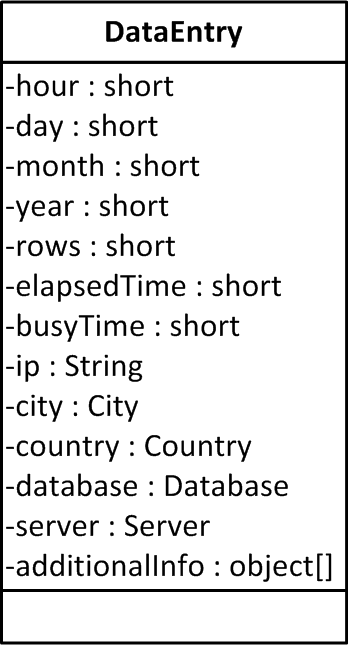
\includegraphics{Pictures/Parts/DataEntry.png}
\end{center}  

\subsubsection*{DataEntry}
The dataEntry which will be written in the warehouse.
It contains 
-hour, day, month, year of the request,
-rows which were read  from the logfile%from the logfile or rows accessed in the original db? %+1, it is not clear
-the elapsed and busy time on the server
-the ip from which the request came
-the type of request
-the database and server which handled the request. %I Thought I'd break this up and make a list
It may contain additional information depending on the actual logfile, as specified in the configuration file. %is this correct?

%\newline\newline doesnt work in empty lines
% \subsubsection*{Java Files}
% The Parser uses java.io.File and a ThreadPool from java.util.

\begin{center}
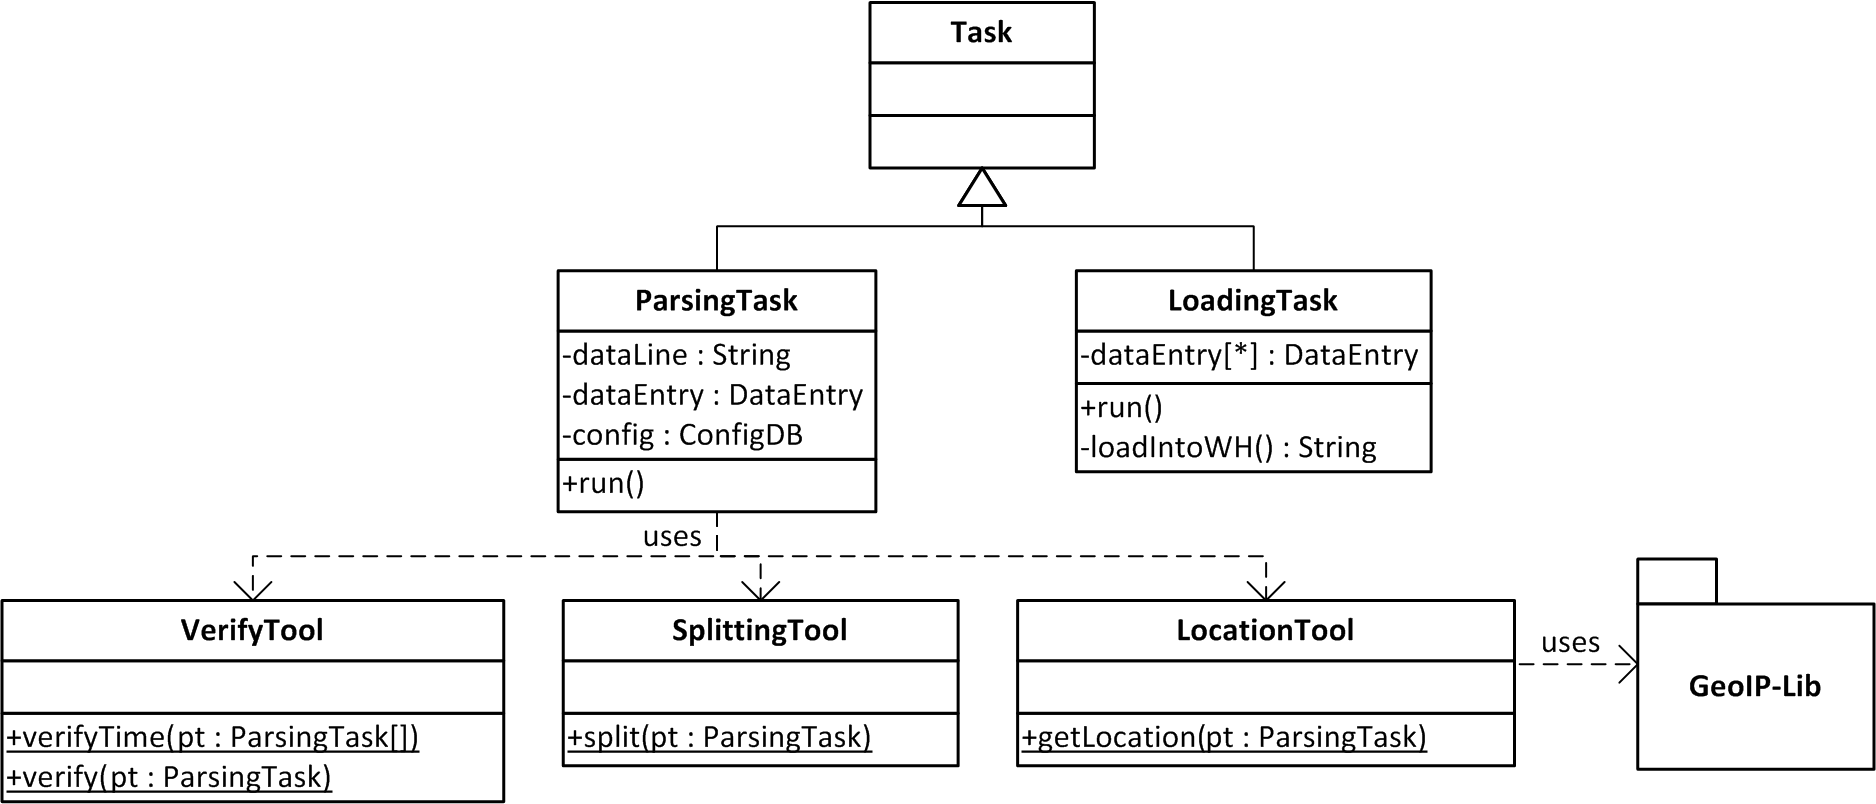
\includegraphics[width=1\linewidth]{Pictures/Parts/TaskTool.png}
\end{center}  

\subsubsection*{ParsingTask}
A ParsingTask is one of the tasks which are created from Parser. It gets a line from the logfile and uses, SplittingTool, VerifyTool
and LocationTool to create a dataEntry which contains the same information. 


\subsubsection*{SplittingTool}
The splitting tool splits the dataLine from its parsingTask and enters the splitted parts into the dataEntry.

\subsubsection*{VerifyTool}
The VerifyTool checks if the dataEntry is correct - if it has a mistake (e.g. Month = 13 or Elapsed Time = -1), it will 
be deleted and the VerifyTool sends an detailed error, which can be displayed elsewhere.

\subsubsection*{LocationTool}
The LocationTool takes the IP from the dataEntry and uses GeoIP-libraries[geo] to determine the city and country of the request.
Those will be added to the dataEntry.


\subsubsection*{LoadingTask}
A loading task is another possible task for the threadPool. It takes a finished dataEntry from the buffer and sends it to the warehouse.

\subsection{Data access tier}

\begin{center}
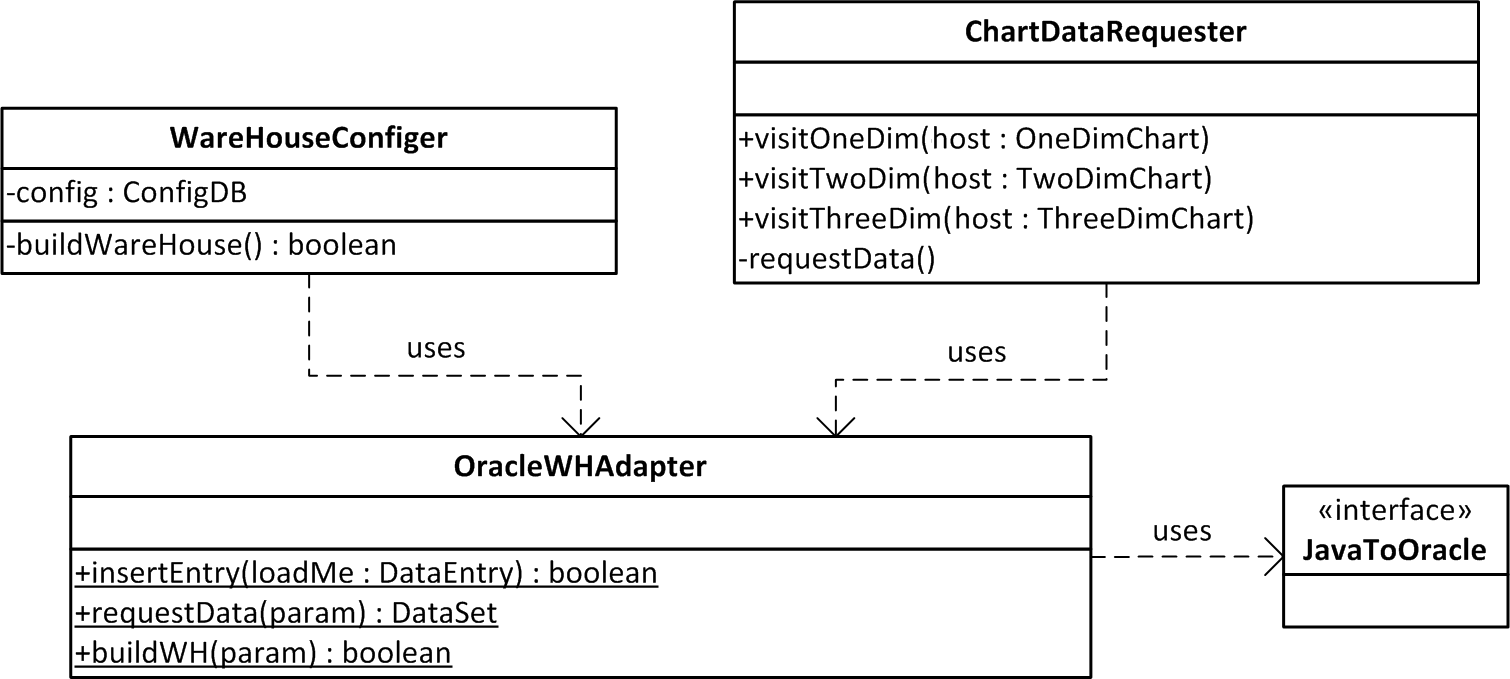
\includegraphics{Pictures/Parts/Data.png}
\end{center} 

\subsubsection*{WareHouseGonfiger}

This Config sends the order to OracleWHAdapter to build the Data Warehouse.

\subsubsection*{ChartDataRequester}

A ChartDataRequester used to send the request to OracleWHAdapter.
There are three types of request:

1) vistOneDim : if the user requestet a Chart with one dimension.

2) vistTwoDim : if the user requestet a Chart with two dimensions.

3) vistThreeDim : the user requestet a Chart with three dimensions.

The response of this class is to build data for the requester.

\subsubsection*{OracleWHAdapter}

After accessing the Database and geting the DataEntry from LoadingTask then OracleWHAdapter will build
the data warehouse in OLAP - Cube form. 
 
\subsubsection*{JavaToOracle}

Is a Library interface, wich makes a connection with a database.

\subsubsection*{Oracle}

A database language. %is it?

geo
 link to the maxmind geoip library in the library section

 
\section{Data warehouse design}

The data warehouse stores all parsed information and creates OLAP-Cubes to achieve fast responses 
for even the most complex of queries.

\subsection{Schema}
The data may be stored in the following schema. If optional functions are implemented and
the warehouses are configured dynamically, the schema may diverge from this.
\begin{center}
%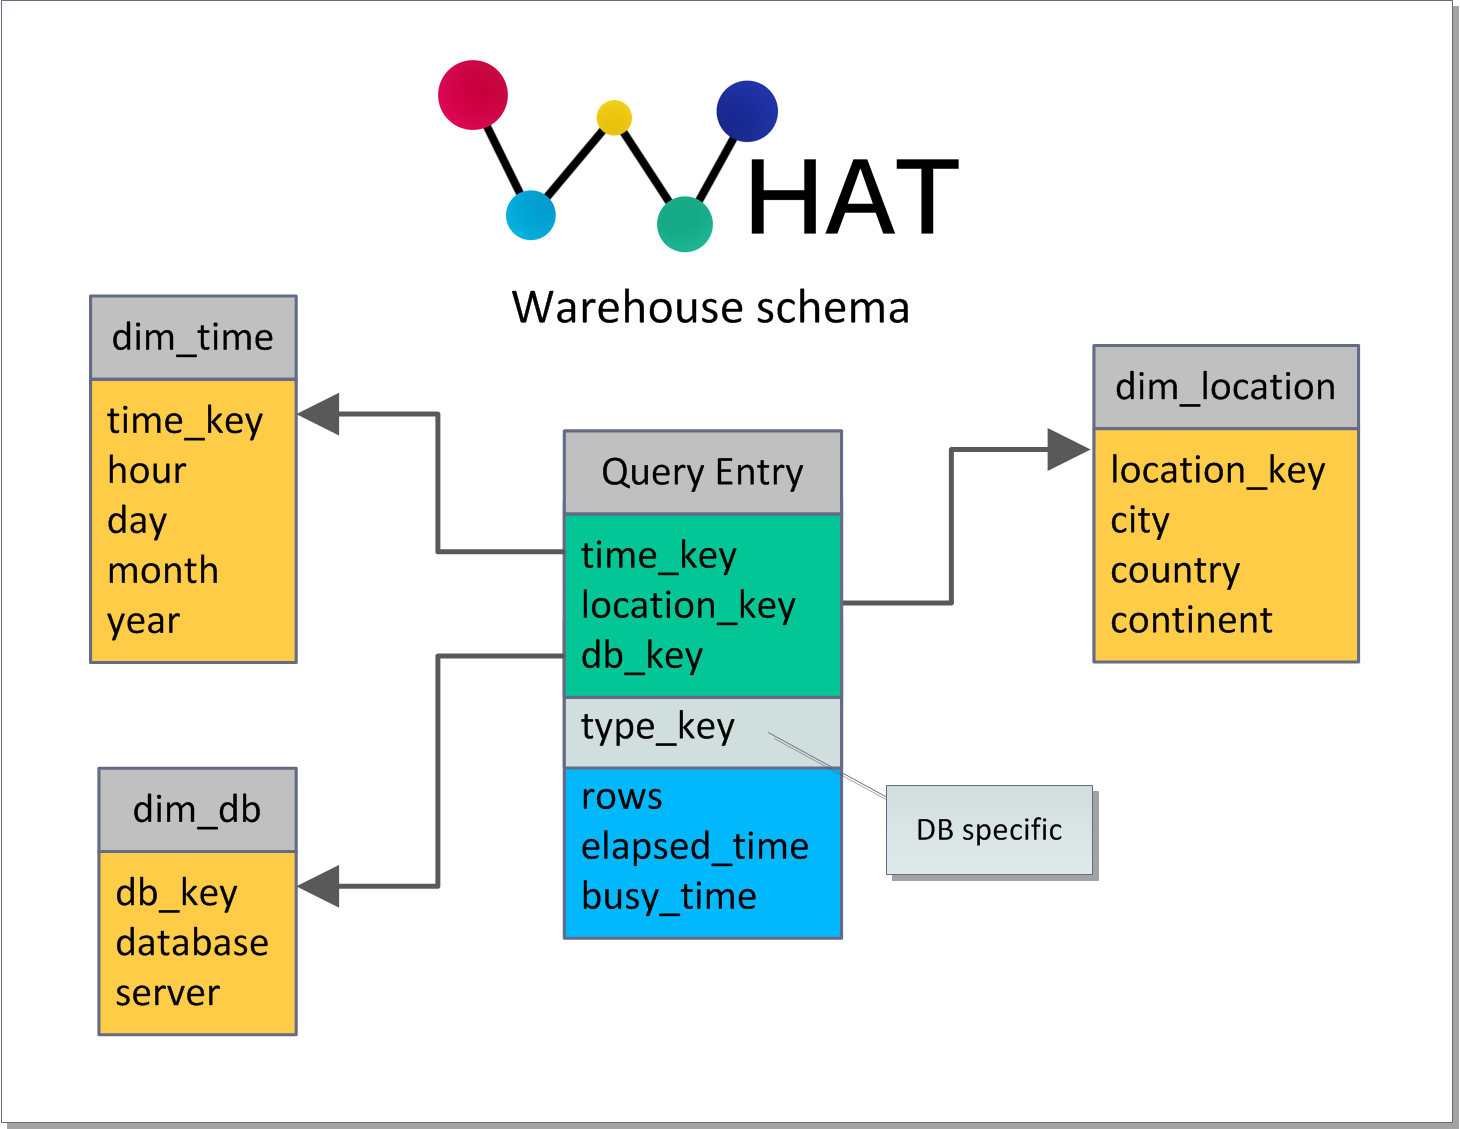
\includegraphics[width=1\linewidth]{Pictures/WHSchema.png}
% or
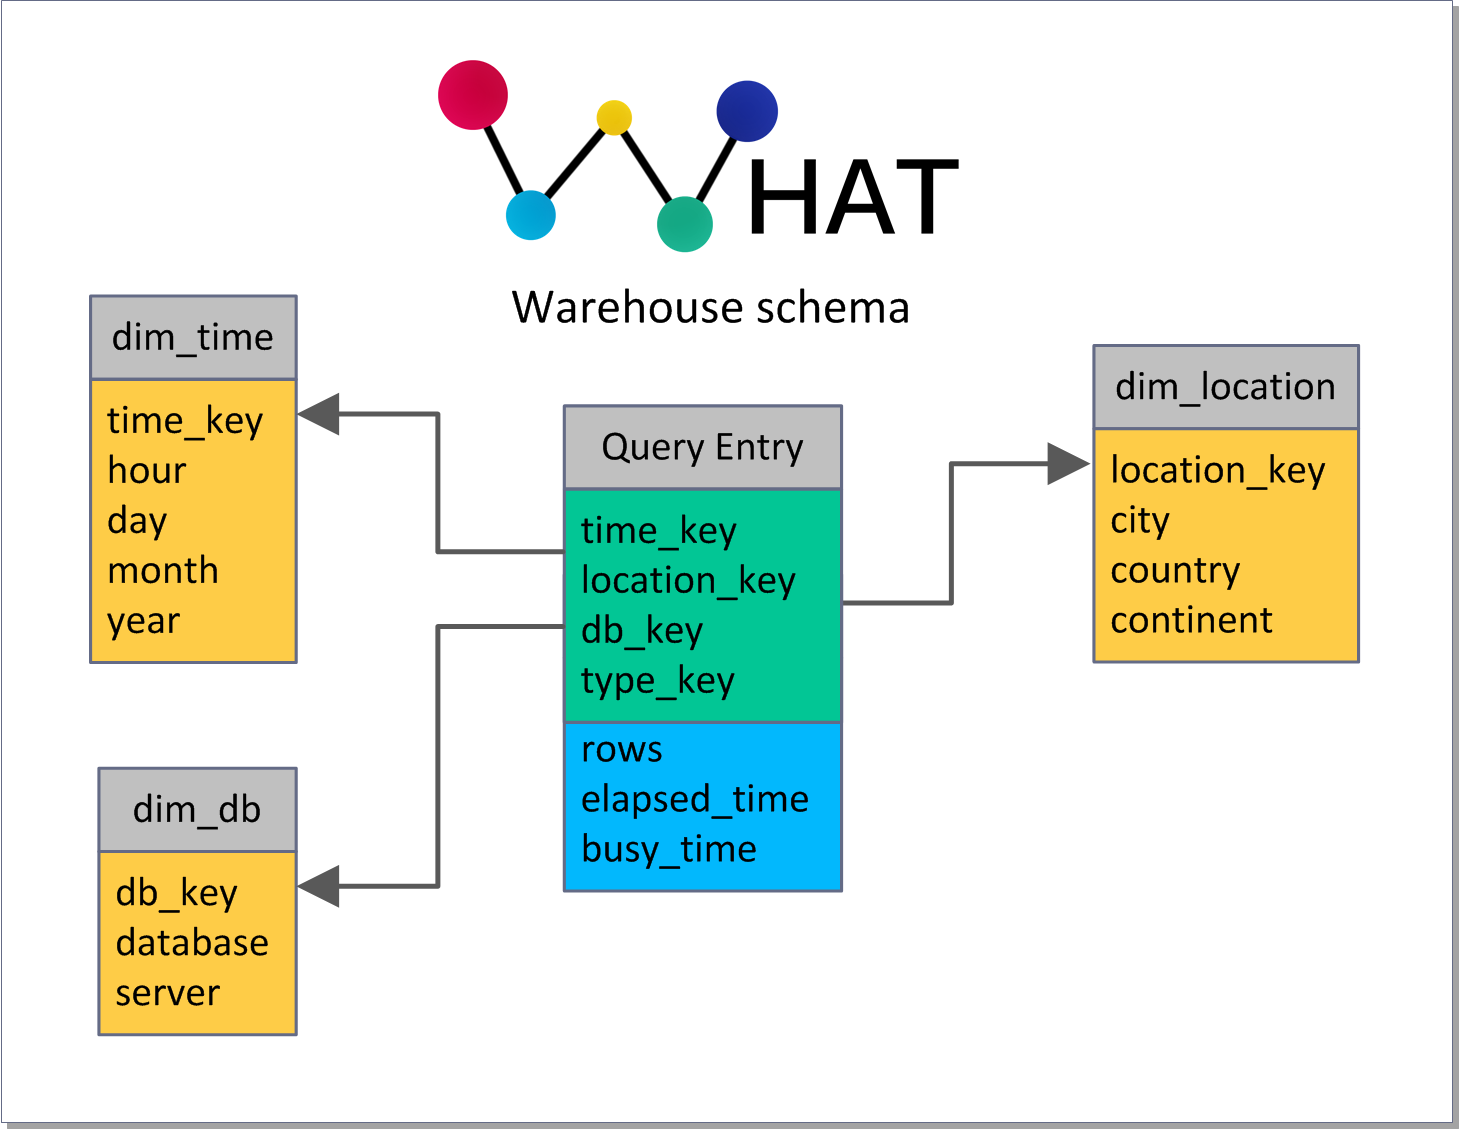
\includegraphics[width=1\linewidth]{Pictures/WHSchema2.png}
\end{center} 


\subsection{Dimension descriptions}
 The only database independent dimensions are time and location. The time dimension is defined by us. The location 
 dimension is given by the GeoIP-lib. (\ref{geo}).
 
 BILD TIME DIMENSION

Other dimensions like database > server, type and maybe others, 
depend on the database operated on, e.g. SkyServer.


\subsection{Measure descriptions}
Measures are for example busy time (CPU time), elapse time and rows. The aggregations stored in the
OLAP-Cubes for this measures are:
\begin{itemize}
 \item sum of their value,
 \item maximum of the value overall in all levels below,
 \item maximum of the values stored for sum in the level below,
 \item number of entries in a level below.
\end{itemize}



  


\section{Sequences}
In this sections the important processes of the system are shown exemplarily. They include a request 
from the web page handled in the web server tier, a call on the facade of the application tier,
a parsing process and a chart request.

\subsection{HTTP request}
A HTTP request is triggered by the user on the web page. This sequence diagram shows
the call of a

\begin{center}
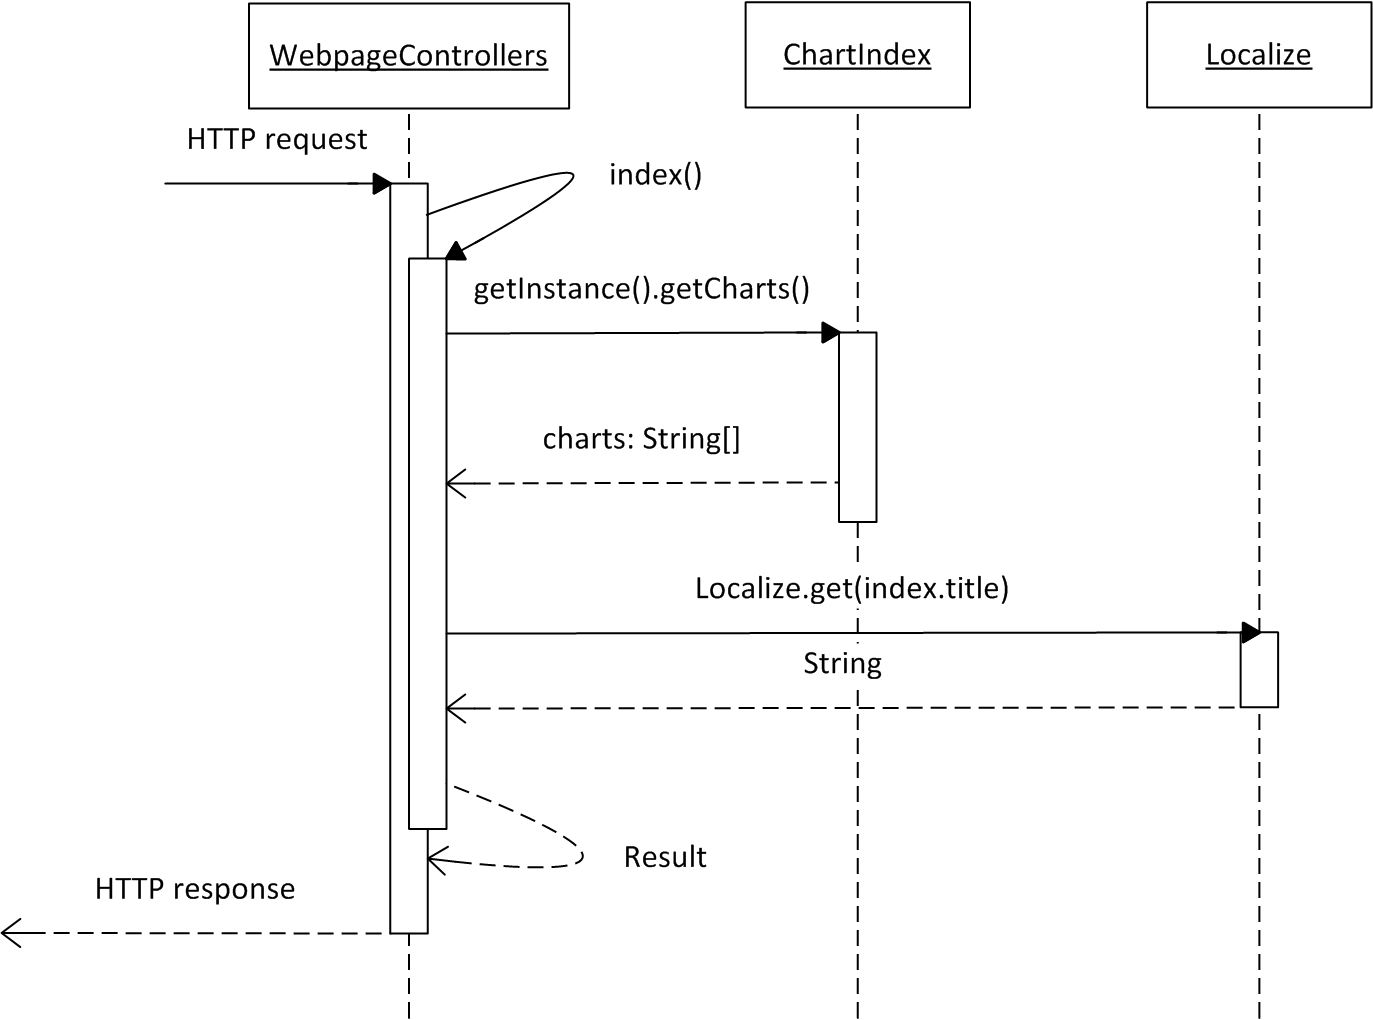
\includegraphics{Pictures/Seq/SeqHTTPRequest.png}
\end{center}


\newpage 
\subsection{Facade call}
In the following sequence diagram a call on the application tier facade is shown 
on the example of a chart request with \texttt{computeChart(..)}.

\begin{center}
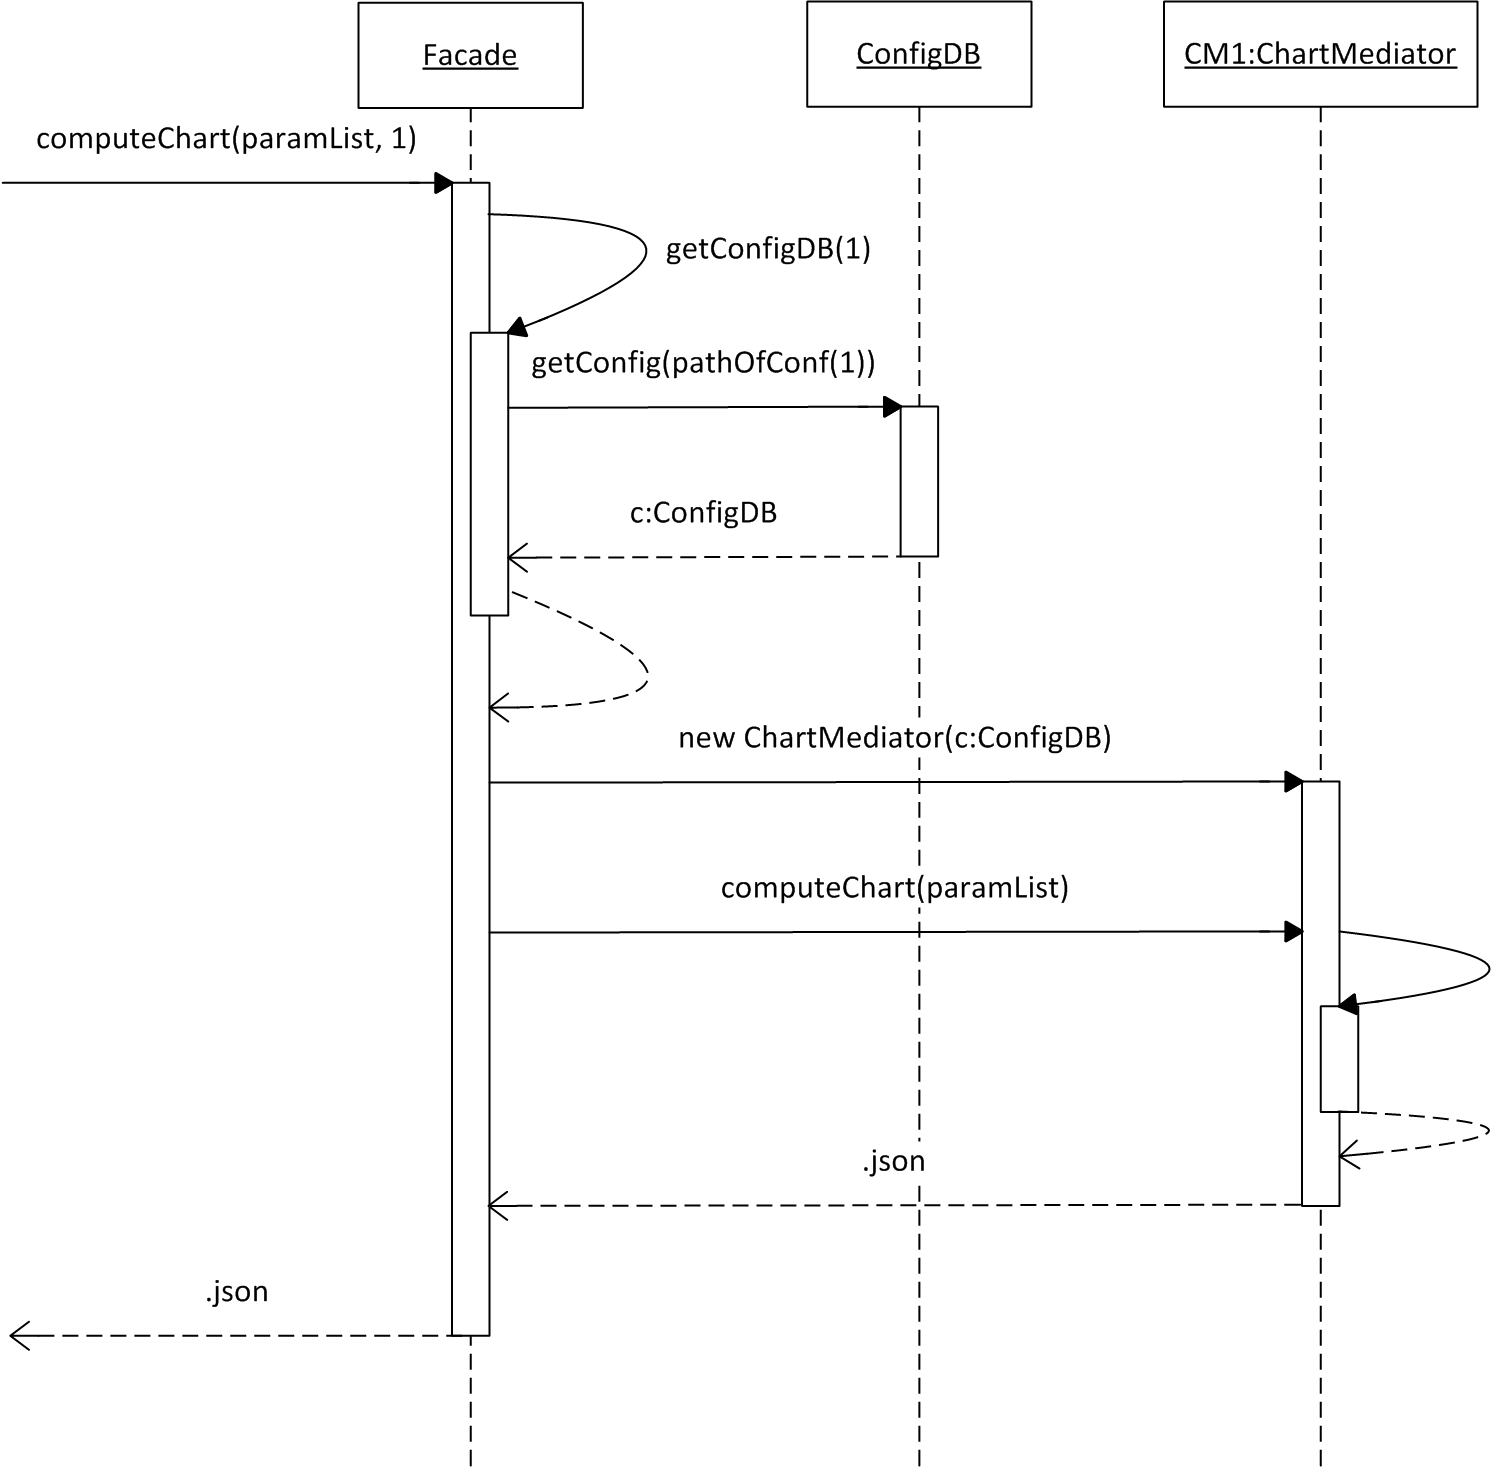
\includegraphics{Pictures/Seq/SeqFacade.png}  
\end{center} 
  


\newpage
\subsection{Chart request}
Sequence diagram of a \texttt{computeChart(..)} call, a chart request, on the ChartMediator.
 
\begin{center}
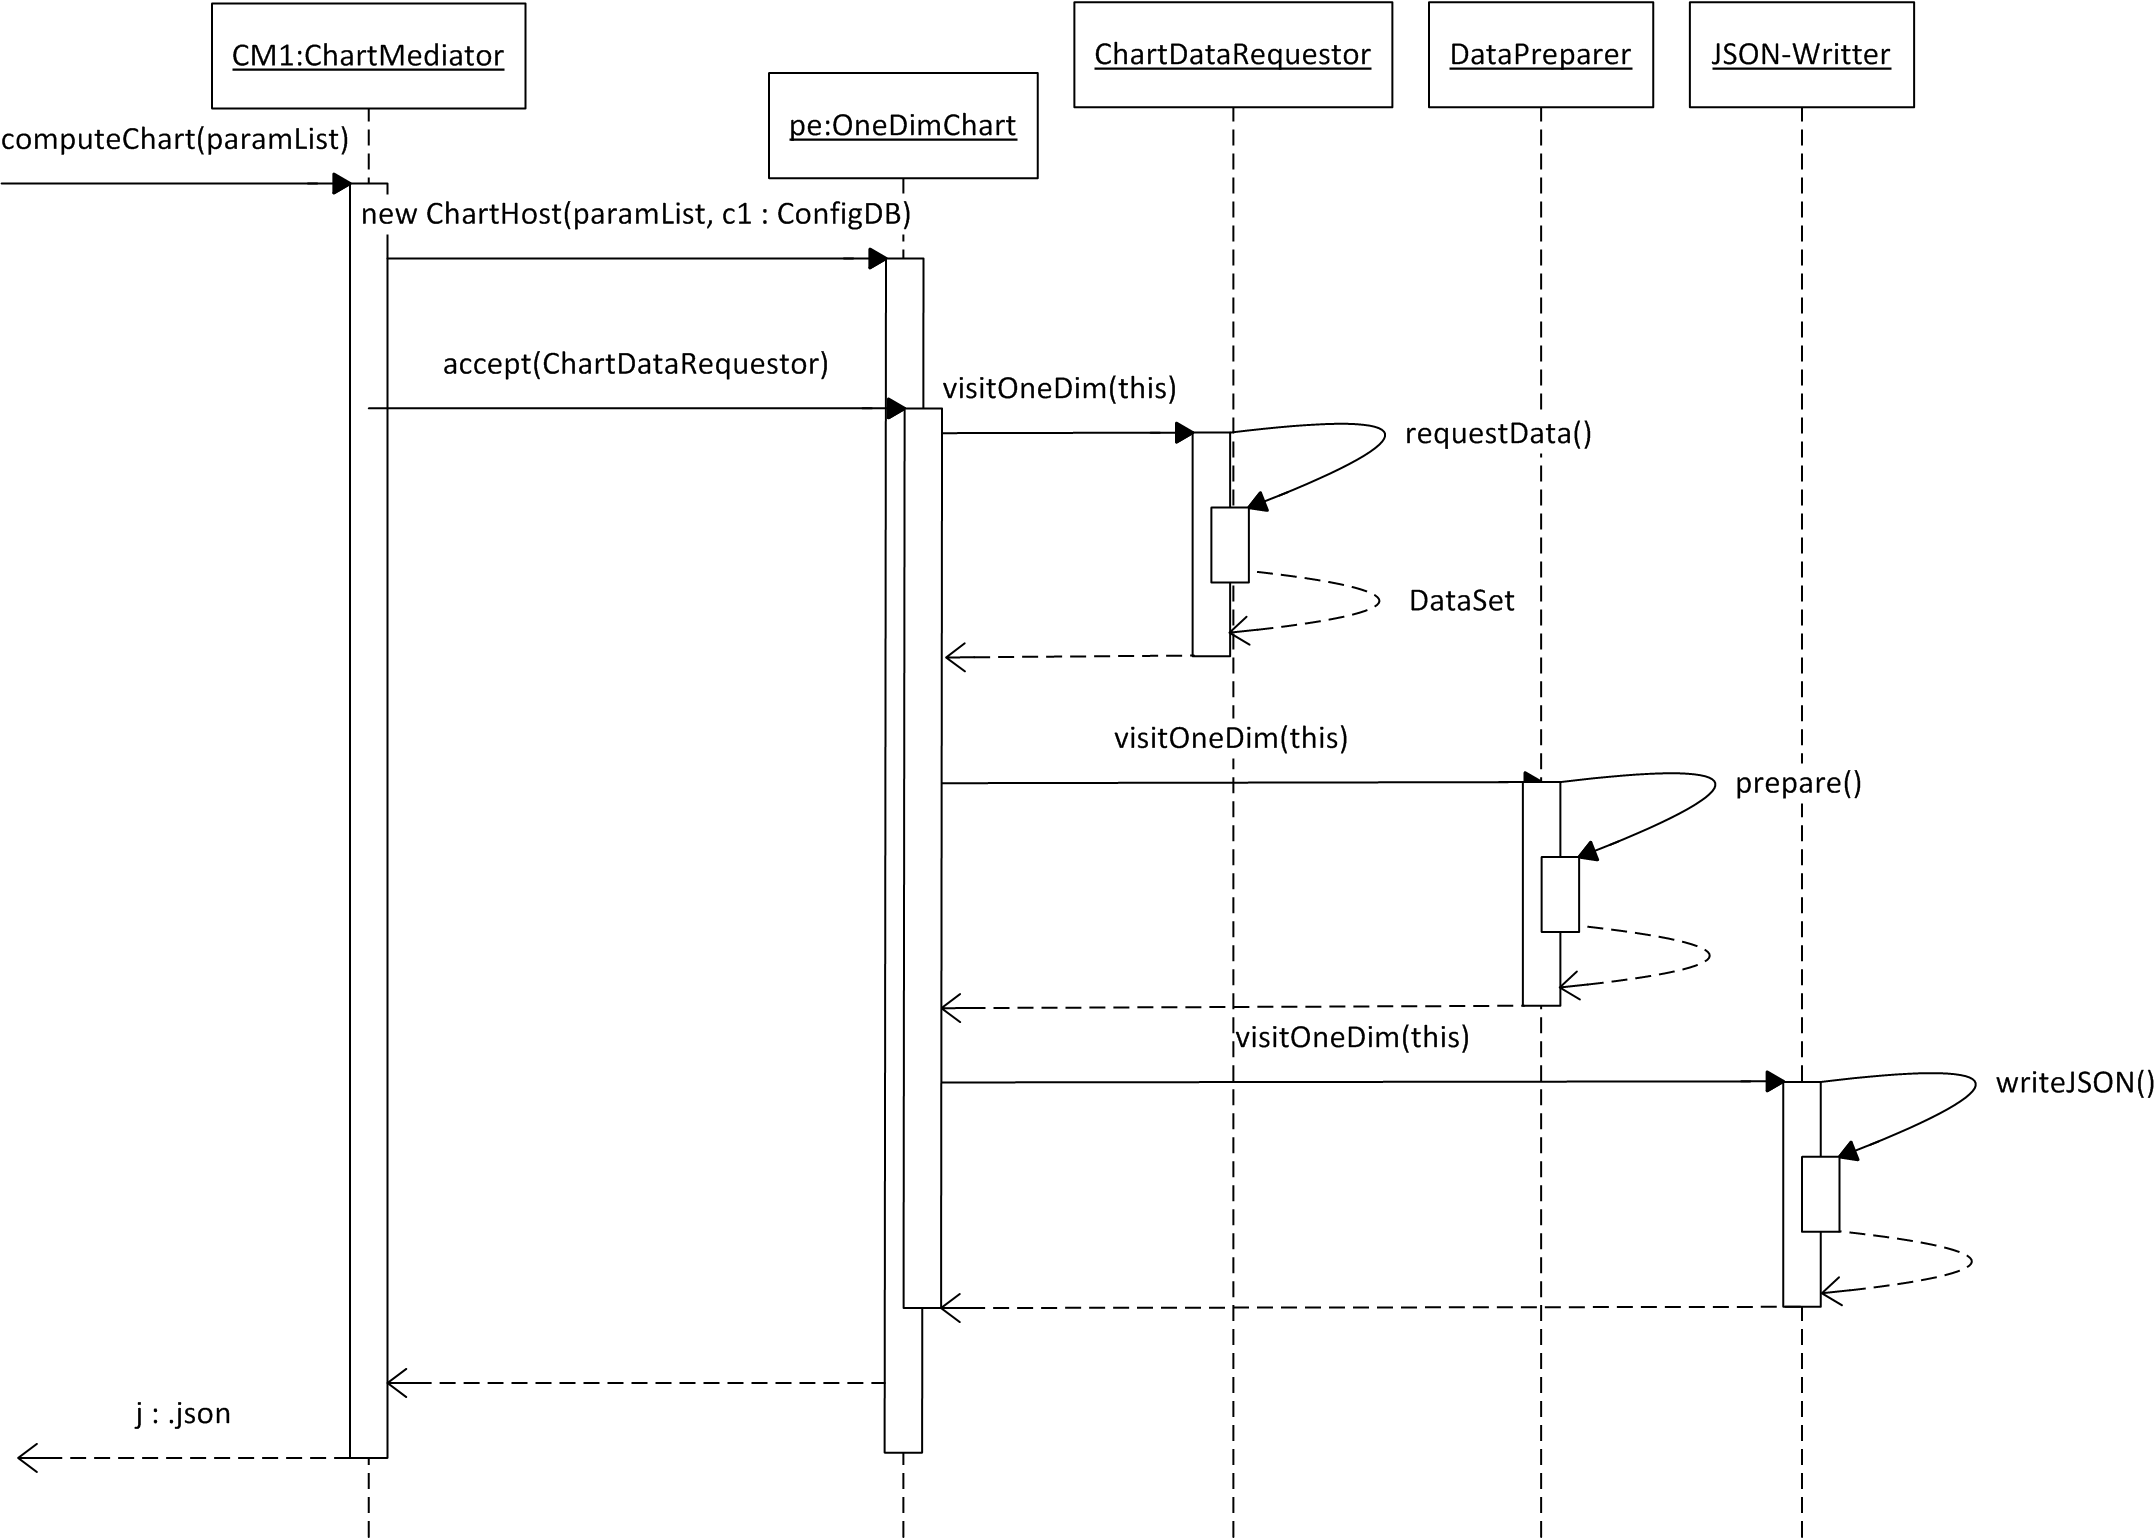
\includegraphics[width=1\linewidth]{Pictures/Seq/SeqChart.png}  
\end{center}
 
\newpage 

\subsection{Parsing} 
%This activity diagram shows the generall work flow of the parsing process of a log file. 
This sequence diagram describes the process after a ParsingTask for one line was created and
called with \texttt{run()}. 
% with the point of view on class interaction.

\begin{center}
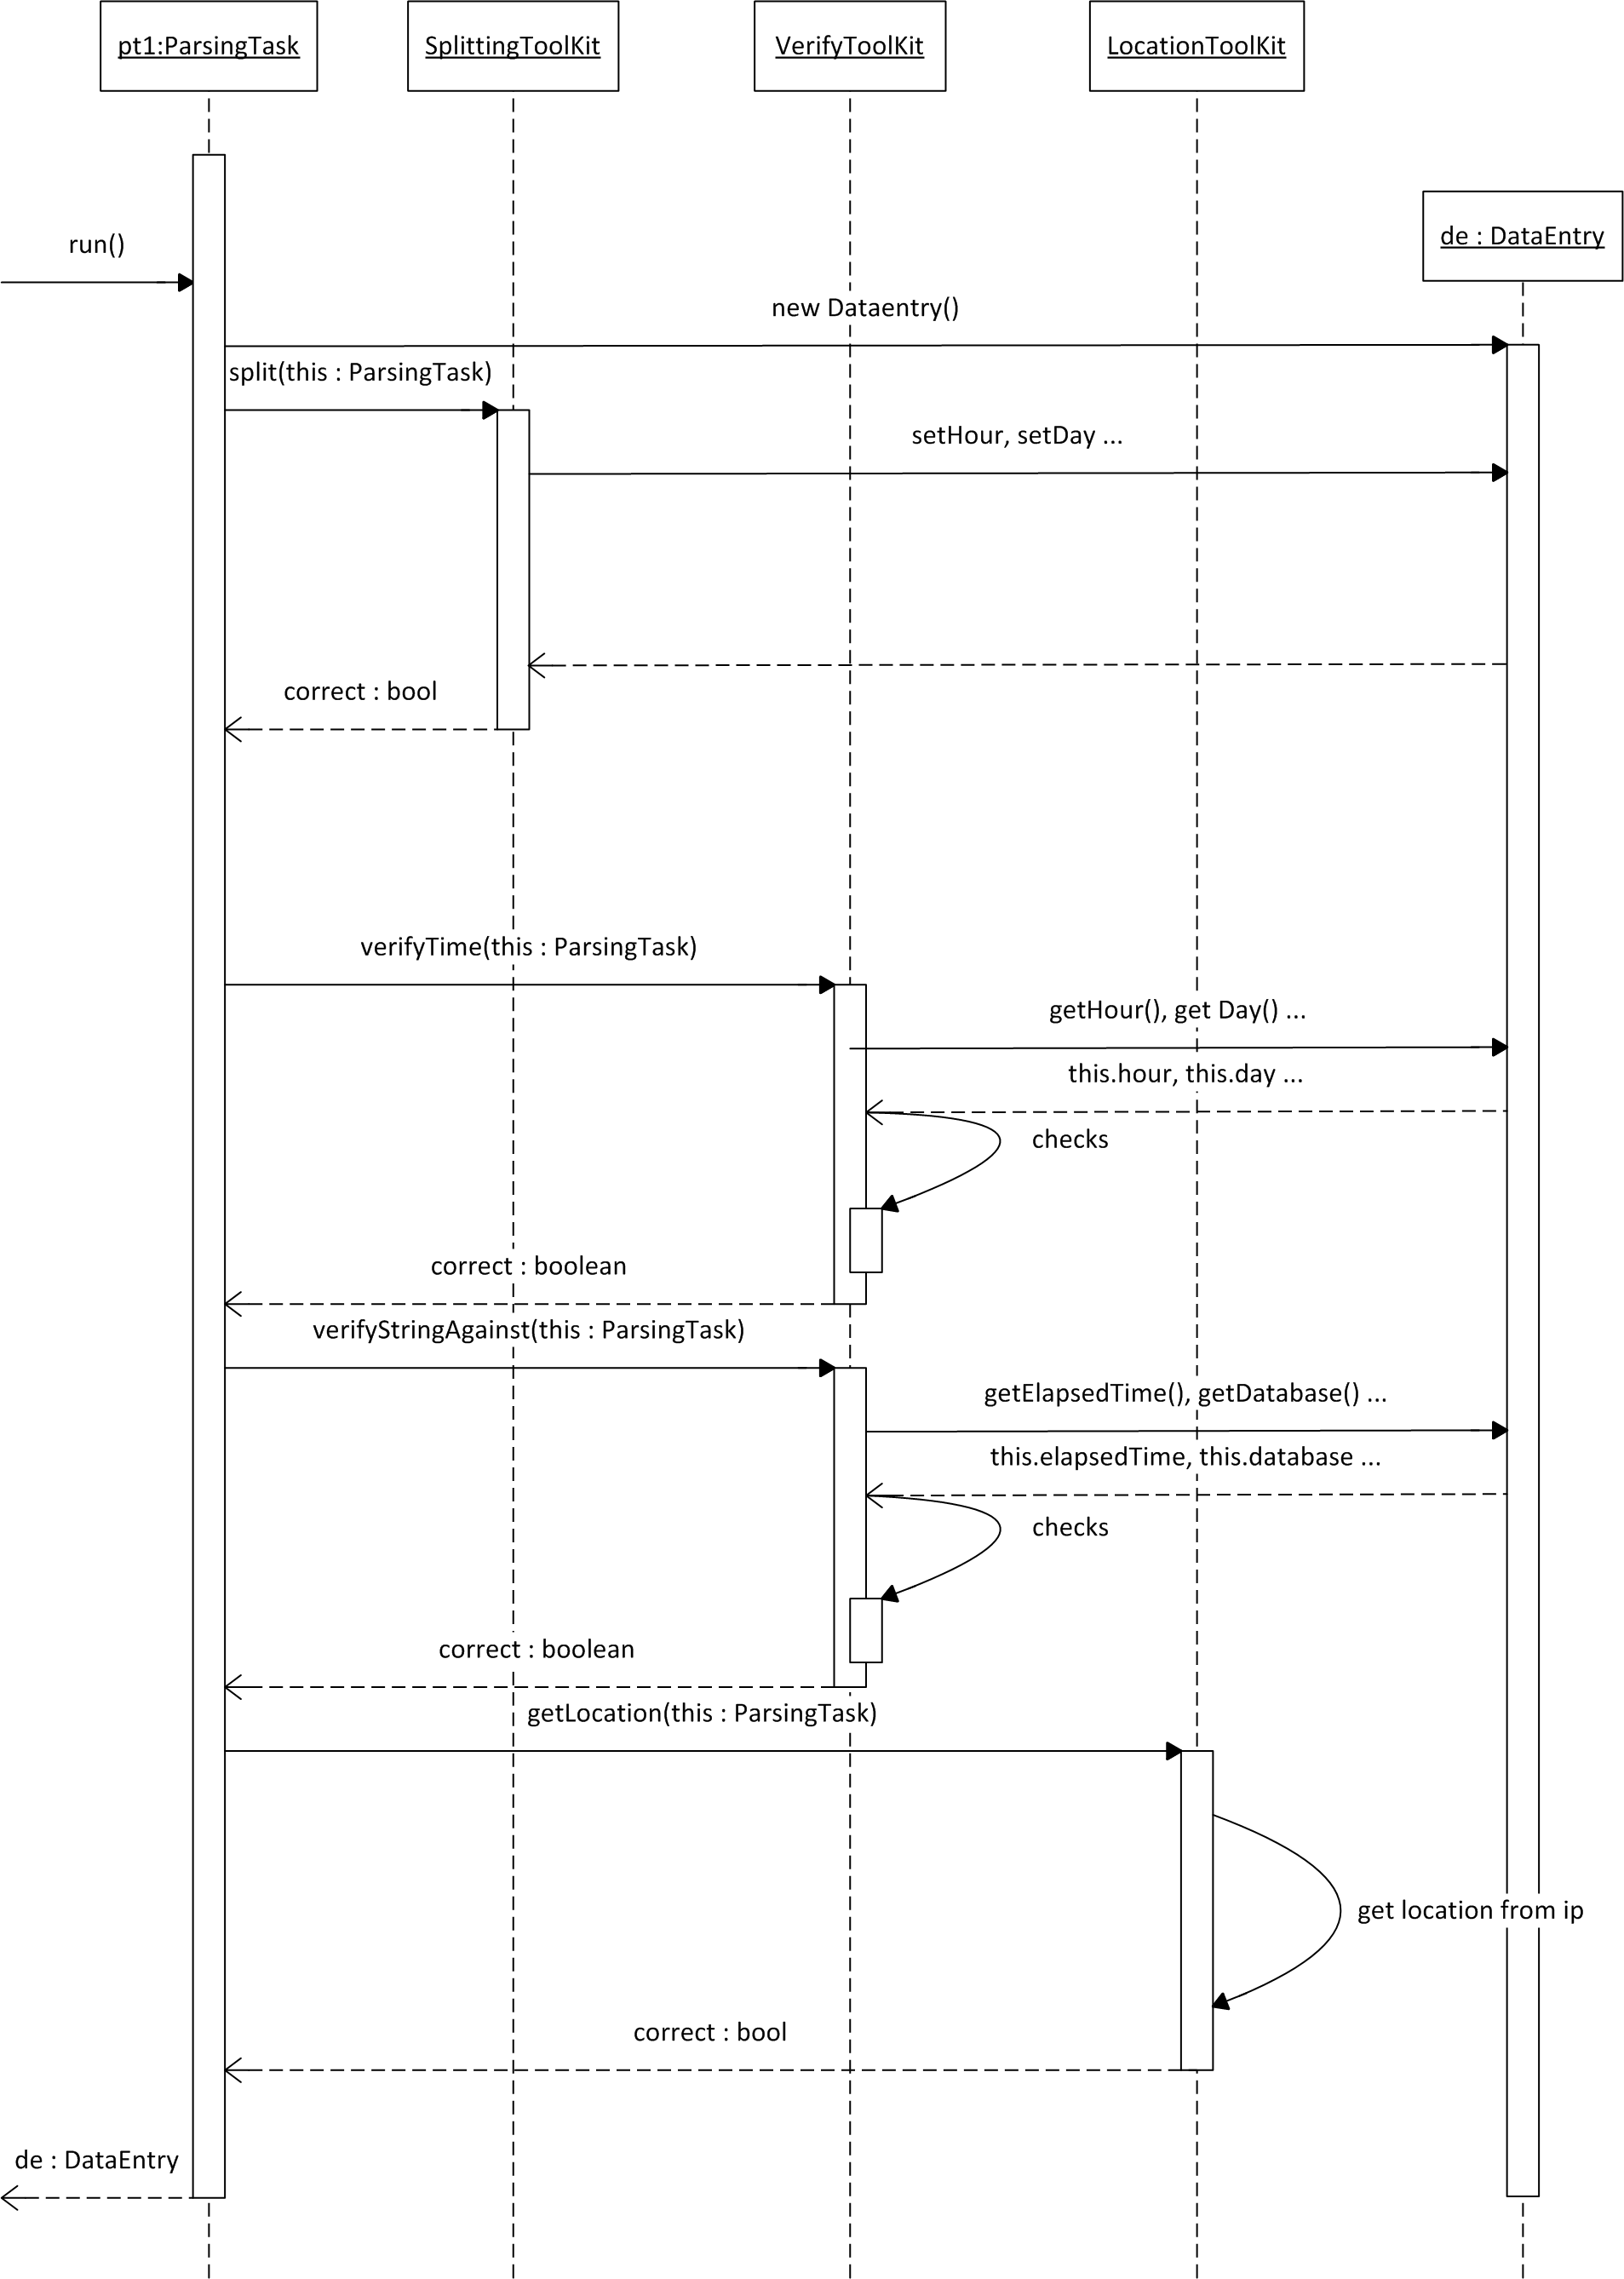
\includegraphics[width=0.8\linewidth]{Pictures/Seq/SeqParser.png}
\end{center}



    

 
\section{Data} % name to be discussed
The program along with its libraries gets compiled to an executable .jar file.
However, it also uses a number of external data.

\subsection{Log files}
Log files are arguably the most important data files our program has to deal with, since it simply
needs them to function properly.

They have to be valid .csv files as well as be consistent with the configuration files specified. 
For more information on configuration files, read on.

\subsection{Configuration files}
This fulfills optional requirements.

The program may work with more database log files than just with these from the SkyServer without 
any modifications to its source code.
However, to achieve this functionality configuration files have to be read. 
A configuration file needs to be written per database.

The configuration file contains, among others, the database schema, the dimensions and 
measures used as well as their types.

Additionally, we will provide a sample configuration file for the skyserver, 
as well as documentation on creating one.


\subsection{Visualization files}
The program dynamically recognizes javascript visualization files during its startup, provided
they are created with our specifications in mind and are either placed in the appropriate directory structure,
or are uploaded through the admin panel.
That said, this allows new chart types, or different visualizations to be created by a user simply by providing
the javascript file. Javascript files have a .js ending.

\subsection{Language files}
Our program keeps language files separate to enable a smooth translation and
maintenance of the graphical user interface.

\subsection{Misc}
Favicons, logos, thumbnails for the chart types are also used.


\section{Libraries}

%    
%!!!!!!!!!!!!!!!!!!!!!!!!!!!!!!!!!!!!!!!!!!!!!!!!!!!!!!!!!!!!!!!!!!!!!!!!!!!%
\end{document}  % END END END END END END END END END END END END END END 
%!!!!!!!!!!!!!!!!!!!!!!!!!!!!!!!!!!!!!!!!!!!!!!!!!!!!!!!!!!!!!!!!!!!!!!!!!!!%
